% TODO: add missing footnotes
% TODO: styling/formatting (e.g., \textit, etc.) 
% TODO: figures, tables, and listings
% TODO: correct bibliography
% TODO: move appendices to end of dissertation?


\chapter{A Case of Kinship: Onomasiological Explorations of \textsc{kinship} in Old Frisian and Old English}
\chaptermark{A Case of Kinship}

\begin{abstract}
This paper describes onomasiological explorations of Old Frisian and Old English lexis in the semantic field of \textsc{kinship} through a novel, digital approach. In connecting Old Frisian lexis, drawn from the Altfriesisches Handwörterbuch (AFWB), to the overarching structure of A Thesaurus of Old English (TOE), a dataset has been created that shares a semantic framework with the one existing for Old English lexis. The connected resources are shared and analysed using the web application Evoke. Statistical data provided by this tool, such as the degree of lexicalization for this field, facilitates comparative analyses of the two historical languages. As this paper demonstrates, the reuse of the onomasiological macrostructure of TOE offers new insights into linguistic and cultural aspects of these two languages and their language communities.
%\keywords{onomasiology, \textsc{kinship}, Old Frisian, Old English, Evoke, digital humanities, linguistic linked data, thesaurus}
\end{abstract}

\section{Introduction}
\label{sect:Stolk2021b:Introduction}

Since its publication in 1995, A Thesaurus of Old English (TOE) has been an asset to research into Old English language and culture. This lexicographic resource captures the early medieval English lexis (c.500–1100), which it does not order alphabetically, like most lexicographic works for Old English do, but onomasiologically: words are organized by means of an overarching topical structure, allowing users to go from meaning to words that express that meaning. In thus positioning words that are similar in meaning close to one another, including the grouping of synonyms, TOE has facilitated numerous word studies and semantic field studies  and its contribution to Old English studies has been met with high praise from scholars (Dance, 1997: 312; Görlach, 1998: 398-399). Hence, the value of an onomasiological ordering of lexis has been demonstrated for Old English. As can be imagined, that value is not limited to this specific language.

Comprehensive thesauri such as TOE, in spite of their value for research, are scarce. The lack of such resources for entire languages is unsurprising: creating a thesaurus takes a considerable amount of time and effort. To illustrate, the creation of TOE (discussed in the contribution by Jane Roberts in this special issue) has taken a team of researchers, themselves drawing from available dictionaries of Old English, over fifteen years (Roberts, 1978). Amongst the languages which have hitherto not yet been captured in a thesaurus is Old Frisian. Yet, in this particular case, the characteristics of this language, combined with resources currently available, may pave the way towards an onomasiological ordering of its lexis in a shorter time than was needed for the creation of a thesaurus of Old English.

Parallels between Old English and Old Frisian have often been drawn and tend to be mentioned explicitly in books that serve as introductions to these languages (see Bremmer, 2009: 125-128; Baker, 2012: 7-8). Indeed, similarities between these ‘sibling languages’ exist on multiple levels – including their lexis. These parallels suggest that an onomasiological marcrostructure designed for Old English may form a good starting point for Old Frisian. Linking Old Frisian lexis to TOE, positioning words and word senses in appropriate locations of its macrostructure, may yield an onomasiological perspective on Old Frisian that is currently absent. Moreover, the placement of Old Frisian senses in this thesaurus is likely to also enable a comparison between these two closely related languages on onomasiological and lexico-semantic levels.

In this article, we describe preliminary work in connecting the Old Frisian lexis to TOE and the use of the results to compare Old Frisian with Old English. For this purpose, we have used the Old Frisian lexis from one particular semantic field, namely that of \textsc{kinship}, mainly represented in TOE by the category “02.03.02 Family/household”.  The connected resources are shared and analysed using the web application Evoke (Stolk, 2018). This application allows researchers to browse and analyse TOE alongside additional content. In addition to discussing our findings in linking up Old Frisian information to the thesaurus, we will present comparative analyses of Old Frisian and Old English provided by the statistical data that Evoke offers, such as the degree of lexicalization of this specific field. Thus, we hope to answer, and nuance, the following questions regarding the semantic fields of \textsc{kinship} in Old Frisian and Old English:

1.	Can the Old Frisian lexis be allocated to the onomasiological macrostructure of TOE?
2.	Can Evoke, in combination with TOE and the linked Old Frisian lexis, offer new insights into linguistic and cultural aspects of Old Frisian and, in contrast with Old Frisian, Old English?

\section{Related Work}
\label{sect:Stolk2021b:RelatedWork}

The number of studies pertaining to Old Frisian linguistics is significantly smaller than those on Old/Middle English or Old/Middle High German (Bremmer, 2007: 55). Most Old Frisian linguistic research investigates a relatively limited aspect of the language or the texts: extensive, comprehensive research is scarce (Bremmer, 1992: 2021). Lexico-semantic Old Frisian studies are almost without exception short treatises on the characteristics of specific lexemes; only a few publications take an onomasiological perspective or comprise an entire semantic field. Although these studies in Old Frisian provide valuable insights into lexical expressions and their meanings, the lexico-semantic research in Old Frisian has hitherto mostly taken a traditional philological approach: they lack empirical or quantitative components.

Research pertaining Old Frisian language is not only sporadic but also often undervalued – especially in the field of historical linguistics Old Frisian is considered to be neglected (Bremmer, 2009: 18; Stroh, 1985: 371; Munske, 2001: xiii; Salmons, 2007: 367). Digital environments for studying Old Frisian are scarce, hampering innovative research (such as comparative studies) of Old Frisian. Recently, however, a digital, lemmatized, and representative corpus of Old Frisian has been published online, a welcome lexicographic resource that can be used by both researchers and students (Van de Poel, 2019). This Corpus Oudfries contains a large sample of the Old Frisian language and can be searched on three linguistic levels (tokens, lemmata, and parts of speech) and on extra-linguistics levels (i.e. dialect and date). At this point in time, the corpus contains 235,462 tokens and 177 text witnesses from 11 manuscripts. Digital resources, such as this corpus and Evoke, provide new means for research into Old Frisian language and culture.

A semantic study of the domain of \textsc{kinship} in Old Frisian has, to our knowledge, not been carried out before, although a limited number of studies are available that investigate individual lexemes and/or certain medieval Frisian legal aspects (Meijers, 1925; Kok, 1947; Boersma, 1961; Sterringa, 1998). For Old English, a comprehensive lexical investigation of kinship terminology has not been conducted either. Various studies have, however, been realized by anthropologists, traditionally the scholars that contributed the most to work on kinship systems and terminology. Lorraine Lancaster (1958), Henry Loyn (1974), and Georg Pfeffer (1987) are among the most influential scholars to have explored Anglo-Saxon kinship terms. Furthermore, certain lexical elements or subdomains within \textsc{kinship} have been investigated for Old English (Spolsky, 1977; Bremmer, 1980; Lowe, 1993; Bajema, 1994; Fischer, 2006; Durkin, 2019).

Relevant semantic word field studies on \textsc{kinship} that should be mentioned are descriptive and comparative studies by Ariane Diepeveen (2003) and Susanne Zeilfelder (2015). Diepeveen provides a diachronic outline how the kinship terms of the (North and West) Germanic languages have evolved over the centuries. She includes almost all Germanic languages in her work, including Old English, but regrettably Old Frisian is absent. Zeilfelder’s onomasiological work mainly focuses on the semantic development and etymology of German. She provides comparisons with and context from other Indo-European languages and to this end also describes Old English and Old Frisian lexemes. However, she does not do this consistently for each sense and/or cognate word. The current study intends to work towards filling this lacuna and to explore how an onomasiological approach, and tools such as Evoke, can facilitate studies of Old Frisian terminology for \textsc{kinship}.

\section{Background: Old Frisian}
\label{sect:Stolk2021b:Background}

Old Frisian is the term used to indicate the earliest version of the Frisian language, written between c.1100–1550. Only a fairly limited number of Old Frisian manuscripts (18) have come down to us, of which the texts are almost entirely juridical in nature.  Besides the major juridical text collections, the largest body of Old Frisian texts consists of administrative documents (charters, wills, deeds), which represents about 50\% of the entire collection of written Old Frisian words. 

The denominator “Old” for Old Frisian suggests that it was more archaic than that of its contemporary neighbouring languages (such as Middle English and Middle High German) and that it was linguistically compatible with, for example, Old English, Old High German, or Old Saxon. Scholars of Old Frisian have investigated the periodization of Old Frisian, which is complicated by the fact that dialectological differences in the language of the textual witnesses concur with the chronological differences: “some linguistic differences have to be interpreted in a chronological sense and some in a dialectological sense” (Versloot, 2004: 256). Rolf Bremmer summarizes the various chronological and dialectological research on Old Frisian and indicates that “the way in which languages are divided into periods depends on the criteria which one chooses in order to establish such periods” (2009: 125).

It has generally been accepted that medieval Frisian texts can be divided into an older and a younger variety (classical/old vs. post classical/late)  and that these periods more or less overlap with the division into regions or dialects. Arjen Versloot indicates that the dialect variety East Old Frisian dates mainly to the period 1300–1450 and was written in the present Dutch province of Groningen and in the German region of East Friesland (2004: 285). The second group originates from the province of Fryslân and was written in the period 1450–1525. He concludes: “Whatever periodisation scheme one prefers, the central conclusion is that the oldest Frisian attestations in the manuscripts represent a language that is fairly compatible with other Old Germanic languages” (2004: 285).


\section{Methodology}
\label{sect:Stolk2021b:Methodology}

In this section we discuss our methodology for linking the Old Frisian lexis to TOE as available in Evoke. In another article in this special issue, Katrien Depuydt and Jesse de Does describe their approach to a similar goal. They have experimented with a (semi-)automated method that matches Old Dutch words from the semantic field of \textsc{kinship} with TOE. Our method, in contrast, involves manually matching dictionary senses to thesaurus categories and can be divided into the following steps:

1.	Identifying Old Frisian lemmata on \textsc{kinship} in the used source dictionary for Old Frisian.
2.	Sense alignment: analysing the different senses of each lemma and matching these senses with a category in TOE or introducing a new category, resulting in a semantic classification.
3.	Processing the alignment into Linguistic Linked Data and importing the work into Evoke.

\subsection{Identifying Old Frisian Lemmata on \textsc{kinship}}
Creating a list of lemmata belonging to the semantic field of \textsc{kinship} was accomplished by manually searching the Altfriesisches Handwörterbuch (AFWB) and marking the words that belong to the semantic field of \textsc{kinship}. The concise dictionary AFWB covers the Old Frisian language from 1200–1550 and was compiled between 1959 and 2008 by Dietrich Hofmann and Anne Popkema. The Old Frisian words are provided with translations into Modern German. The compilers of AFWB did not intend the dictionary to be comprehensive, but included as many lemmata and sense distinctions as needed for its use as a reading companion to Old Frisian texts (AFWB: xxiii-xxiv). The dictionary contains 11,254 headwords, of which 247 (2\%) were selected as they belonged to the semantic field of \textsc{kinship} and were therefore eligible for linking to the TOE.

A dictionary entry in the AFWB has the following format: the lemmata are printed in bold, a reference to dialect is printed in superscript (WL or OL), followed by the part of speech category, senses, sources (there is no indication which sense was found in which text source), composites and cross-references.

frouwe, frowe, frouWL f. 1) Frau; 2) Ehefrau; 3) Edelfrau, Fürstin; 4) Herrin; 5) die Jungfrau Maria; 6) Schwiegermutter –
Bas, BBr-D, BDg-U, BEm-E1E2, BFi-F, Bgr-J, BHm-J, BHua-H, BHub-H, (...). 
Komp.: ethelinges- , gā- , hāved- , hērskipes- , hūs- , jest- , jung- , klāster- , londes- , lond- , munekfrouwe

The head word is followed by subsidiary lemmata that pertain to phonological and/or orthographical (and often dialectal) variations of the head word. The lemmata within an entry are arranged in chronological order, which means that the earliest attestation is always the head word. In our methodology, the first lemma was selected for inclusion in the alignment. Thus, the earliest Old Frisian word forms have been imported into Evoke. The compilers of the AFWB have harmonized the spellings of many word forms to ensure that lexemes belonging together can easily be retrieved. 

An AFWB lemma can have multiple senses, which are distinguished by numbers. Frequently, however, the senses of a lemma also contain commas that seem to indicate slightly overlapping meanings. Examples are: efterswesterling – “Andergeschwisterkind, Verwandter im dritten Grade” [second cousin, third-degree relative] and niftakind – “Grosskind, kind des Nichten” [grandchild, niece’s child]. For the scope of the present study, we decided to consider these descriptive meanings as elaborations rather than distinct senses.

\subsection{Sense Alignment}
Three spreadsheets were developed in order to facilitate data entry and subsequent data conversion into Linguistic Linked Data, the interoperable data format used by Evoke. These spreadsheets represent the three main elements that are to be captured: lexical entries, senses, and concepts. Fig. \ref{fig:Stolk2021b:Fig1} shows the sheet for lexical senses. This sheet, which is pivotal in the alignment of the Old Frisian words and their senses with TOE, provides local identifiers for the current word (B) and for this word in a specific sense (A), the head word (D), the language code according to ISO 639 (E; here “ofs” for Old Frisian), and the identifier for the semantic category (F) in which the sense is to be positioned. The identifier of a category can be either an existing one from TOE (a web address also referred to as an IRI) or a newly coined category identified by a number and defined on the sheet for lexical concepts — including where this newly defined category fits into the TOE taxonomy.

\begin{figure}[htbp]
	\framebox[\textwidth]{
		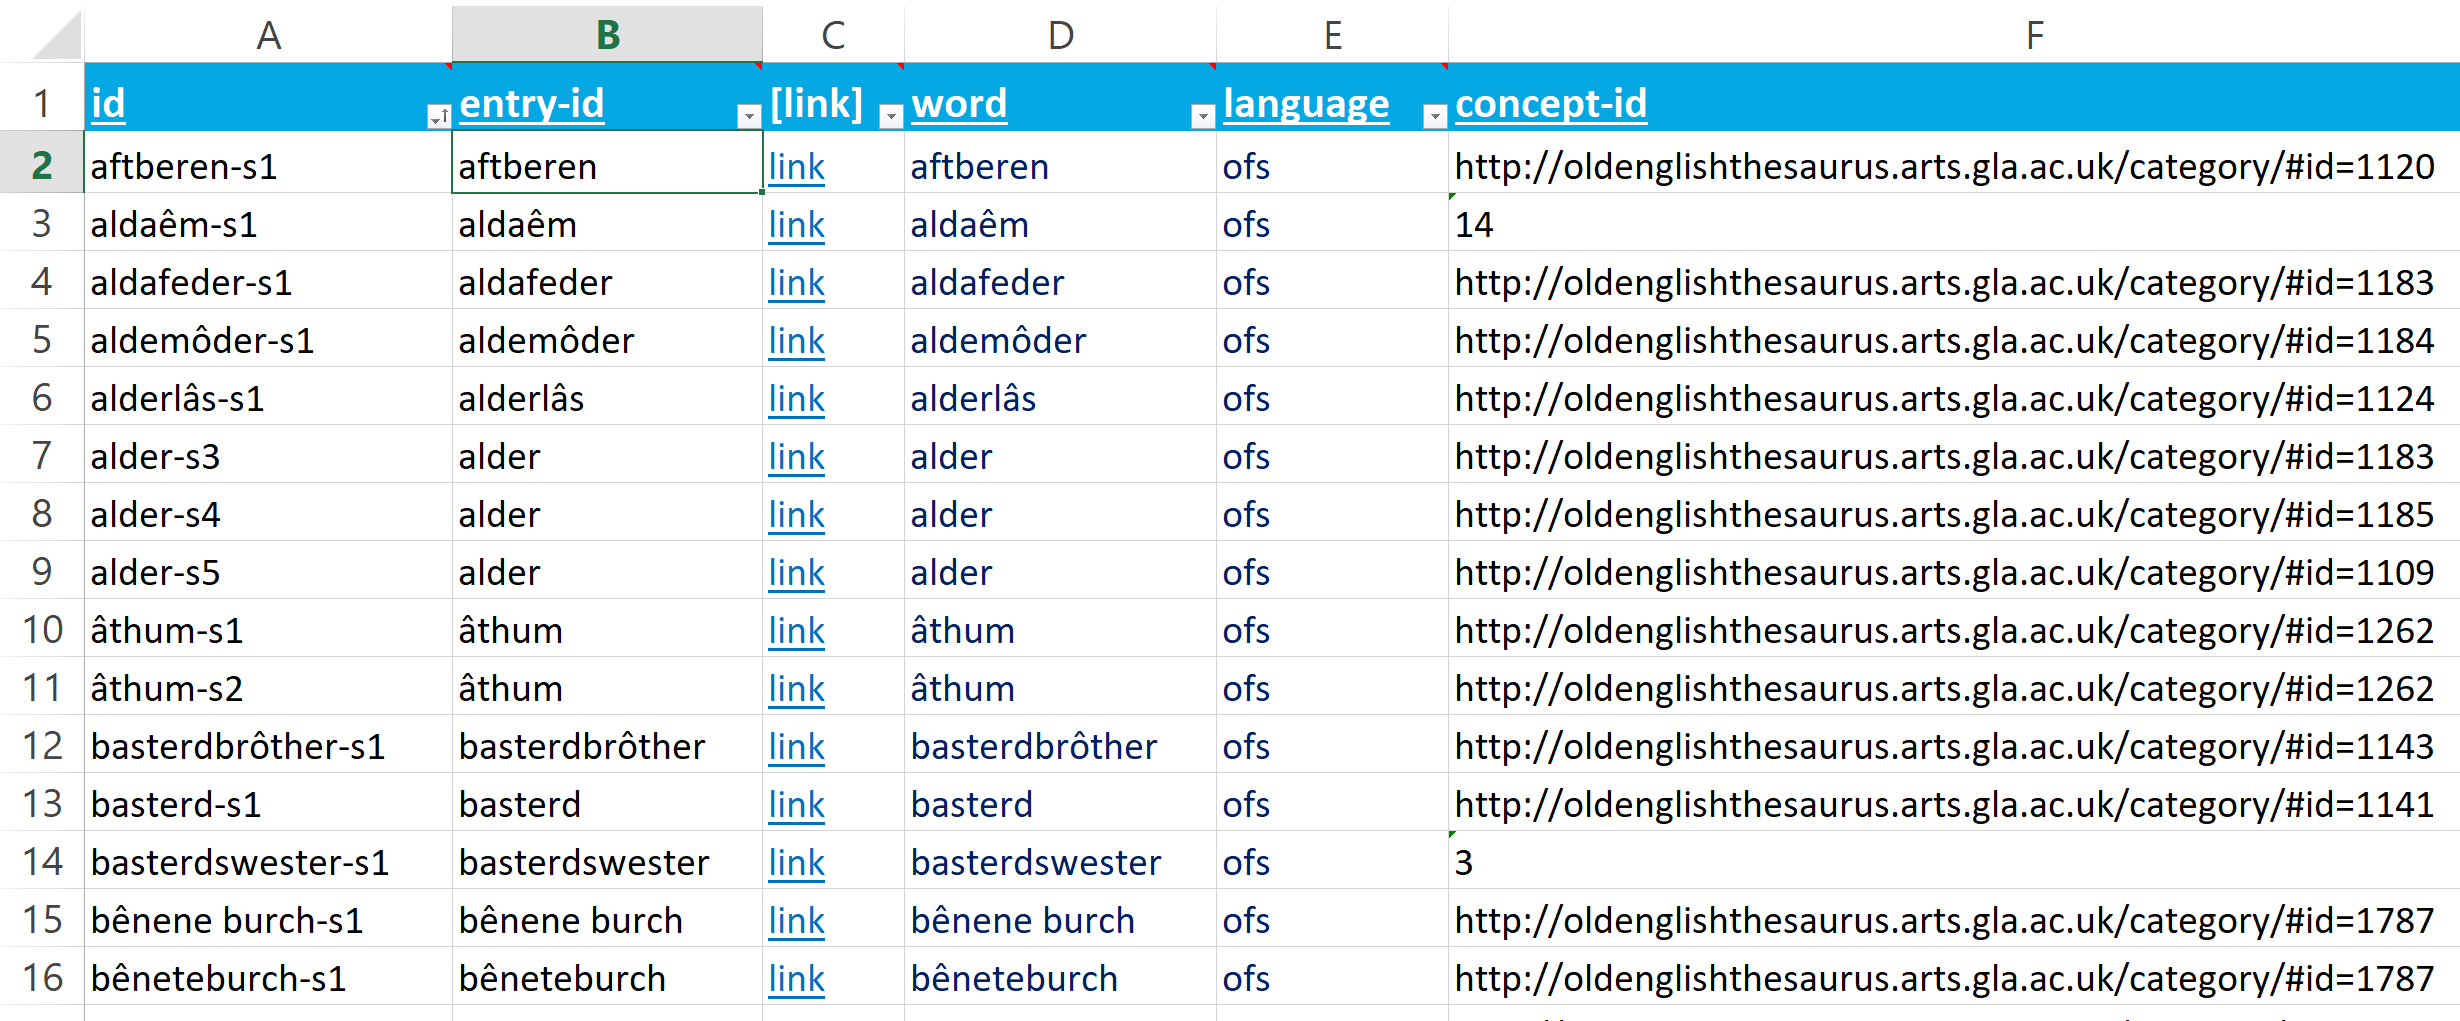
\includegraphics[width=\textwidth]{Stolk2021b/fig/Fig1.png}
	}
	\caption[]{\label{fig:Stolk2021b:Fig1} Spreadsheet used in recording Old Frisian senses and the concepts to which they relate.}
\end{figure}

The following activities are involved in assigning the senses of the Old Frisian lexemes to appropriate categories in TOE (either existing ones or new ones that add a further degree of specialization):

\begin{itemize}
    \item Record the lemma and its Modern German senses in the spreadsheets.
    \item Translate Modern German sense definitions into Modern English.
    \item Locate suitable TOE categories by
    \begin{enumerate}[label=(\alph*)]
        \item browsing the taxonomy of TOE
        \item searching for categories that contain keywords from the translated Modern English definitions of the lemma, and
        \item searching for the Old English cognates, if any, and marking the TOE categories at which they are positioned. 
    \end{enumerate}
    \item Record matching TOE categories in the spreadsheets. When no matching TOE category is available for a sense, create a new category in the spreadsheet and position that category in the TOE taxonomy by recording its superordinate category.
    \item Determine whether Old English cognates appear in more than one category, since this could imply that the Old Frisian lexeme under investigation would also have to be assigned to these other categories in order to facilitate contrasting the two languages. 
\end{itemize}


\subsection{Processing the Alignment for Use in Evoke}
In order to transform the three spreadsheets to Linguistic Linked Data, we have employed the conversion tool OpenRefine along with its RDF plugin. The conversion logic for these sheets has been made publicly available.  Each row in the sheet for lexical senses is transformed into an instance of a data element as defined in OntoLex, an interoperable model that has been designed specifically for capturing linguistic data, such as lexical entries and their senses.  The resulting Linguistic Linked Dataset has been imported into the online repository of Evoke.

\section{Results}
\label{sect:Stolk2021b:Results}

Numbers on the created dataset, which is now publicly available in Evoke, are as follows: 280 lexical senses on \textsc{kinship}, from 247 Old Frisian lemmata, have been aligned with TOE categories (see Appendix 2).  The majority of these senses have been allocated to the semantic field “02.03.02 Family/household”, as the following overview shows:

\begin{verbatim}
    02.01 Existence, life (id: 661)                  21 senses
    02.03 Humankind (id: 1059)                       2 senses + those in 
                                                     subfields (below)
        02.03.01 People (id: 1065)                       31 senses
        02.03.02 Family/household (id: 1108)             215 senses
    12.09 Marriage, state of marriage (id: 18602)    11 senses
\end{verbatim}

\noindent Since “02.03.02 Family/household” represents the core of Old Frisian terminology on \textsc{kinship}, this case study concentrates its onomasiological analyses on this semantic field.

Old Frisian senses placed under “02.03.02 Family/household” have either been allocated to already existing TOE categories (132 senses to 70 TOE categories) or to categories newly introduced into the TOE taxonomy (83 senses to 57 new categories). Originally, the field “02.03.02 Family/household” contained a total of 175 categories with 324 recorded Old English senses. An overview of these numbers is provided in Table \ref{table:Stolk2021b:item-counts}. A substantial number of categories from this field in the expanded taxonomy have solely Old Frisian or solely Old English senses assigned to them (162 out of a total of 232 categories, or 70\%). In the field of \textsc{kinship}, then, the recorded vocabularies of these kindred languages contain many differences in denotations and nuances of words. We will elaborate on some of the more apparent differences in our discussion of the distribution of Old Frisian lexis over the various semantic subfields of “02.03.02 Family/household”, in section \ref{sect:Stolk2021b:OnomasiologicalDistrubtionOverCategories}.

\begin{table}[ht]
	\normalsize
	\center
	\setlength\tabcolsep{0.5em}
	\begin{tabular}{p{8.9cm}cc}
	\toprule
	                  & \textbf{Old English} & \textbf{Old Frisian} \\
    \midrule
    number of lemmata & 294         & 200 \\
    number of senses  & 324         & 215 \\
    number of categories w/ senses allocated to them & 175 & 127 \\
    \midrule
	\end{tabular}
	\caption{Item counts within the field “02.03.02 Family/household”.\label{table:Stolk2021b:item-counts}}
\end{table}


\subsection{Locating Old Frisian Words, Their Synonyms, and Cognates}
As a consequence of the categorization of the Old Frisian lexis with the macrostructure of TOE, the web application Evoke can offer scholars a seamless integration of Old English and Old Frisian lexis for the field of \textsc{kinship}. Thus, not only words for a given concept can be obtained for either language, but also synonyms and possible translations between them. Such an integrated overview of this information can be activated by selecting both relevant datasets in Evoke (i.e. TOE and the Old Frisian dataset newly created for this research). When subsequently opening a category such as “02.03.02.03.03 Forefather, ancestor” in the user interface of the application,  it is revealed which words were used to express this concept in both Old Frisian and Old English. The list presented in Fig. \ref{fig:Stolk2021b:Fig2} shows six different Old English words for this concept (including ǣrfæder and ieldra) compared to three for Old Frisian (viz. alder, forefeder, forefirdera). These words are grouped by language and sorted alphabetically.
 
\begin{figure}[htbp]
	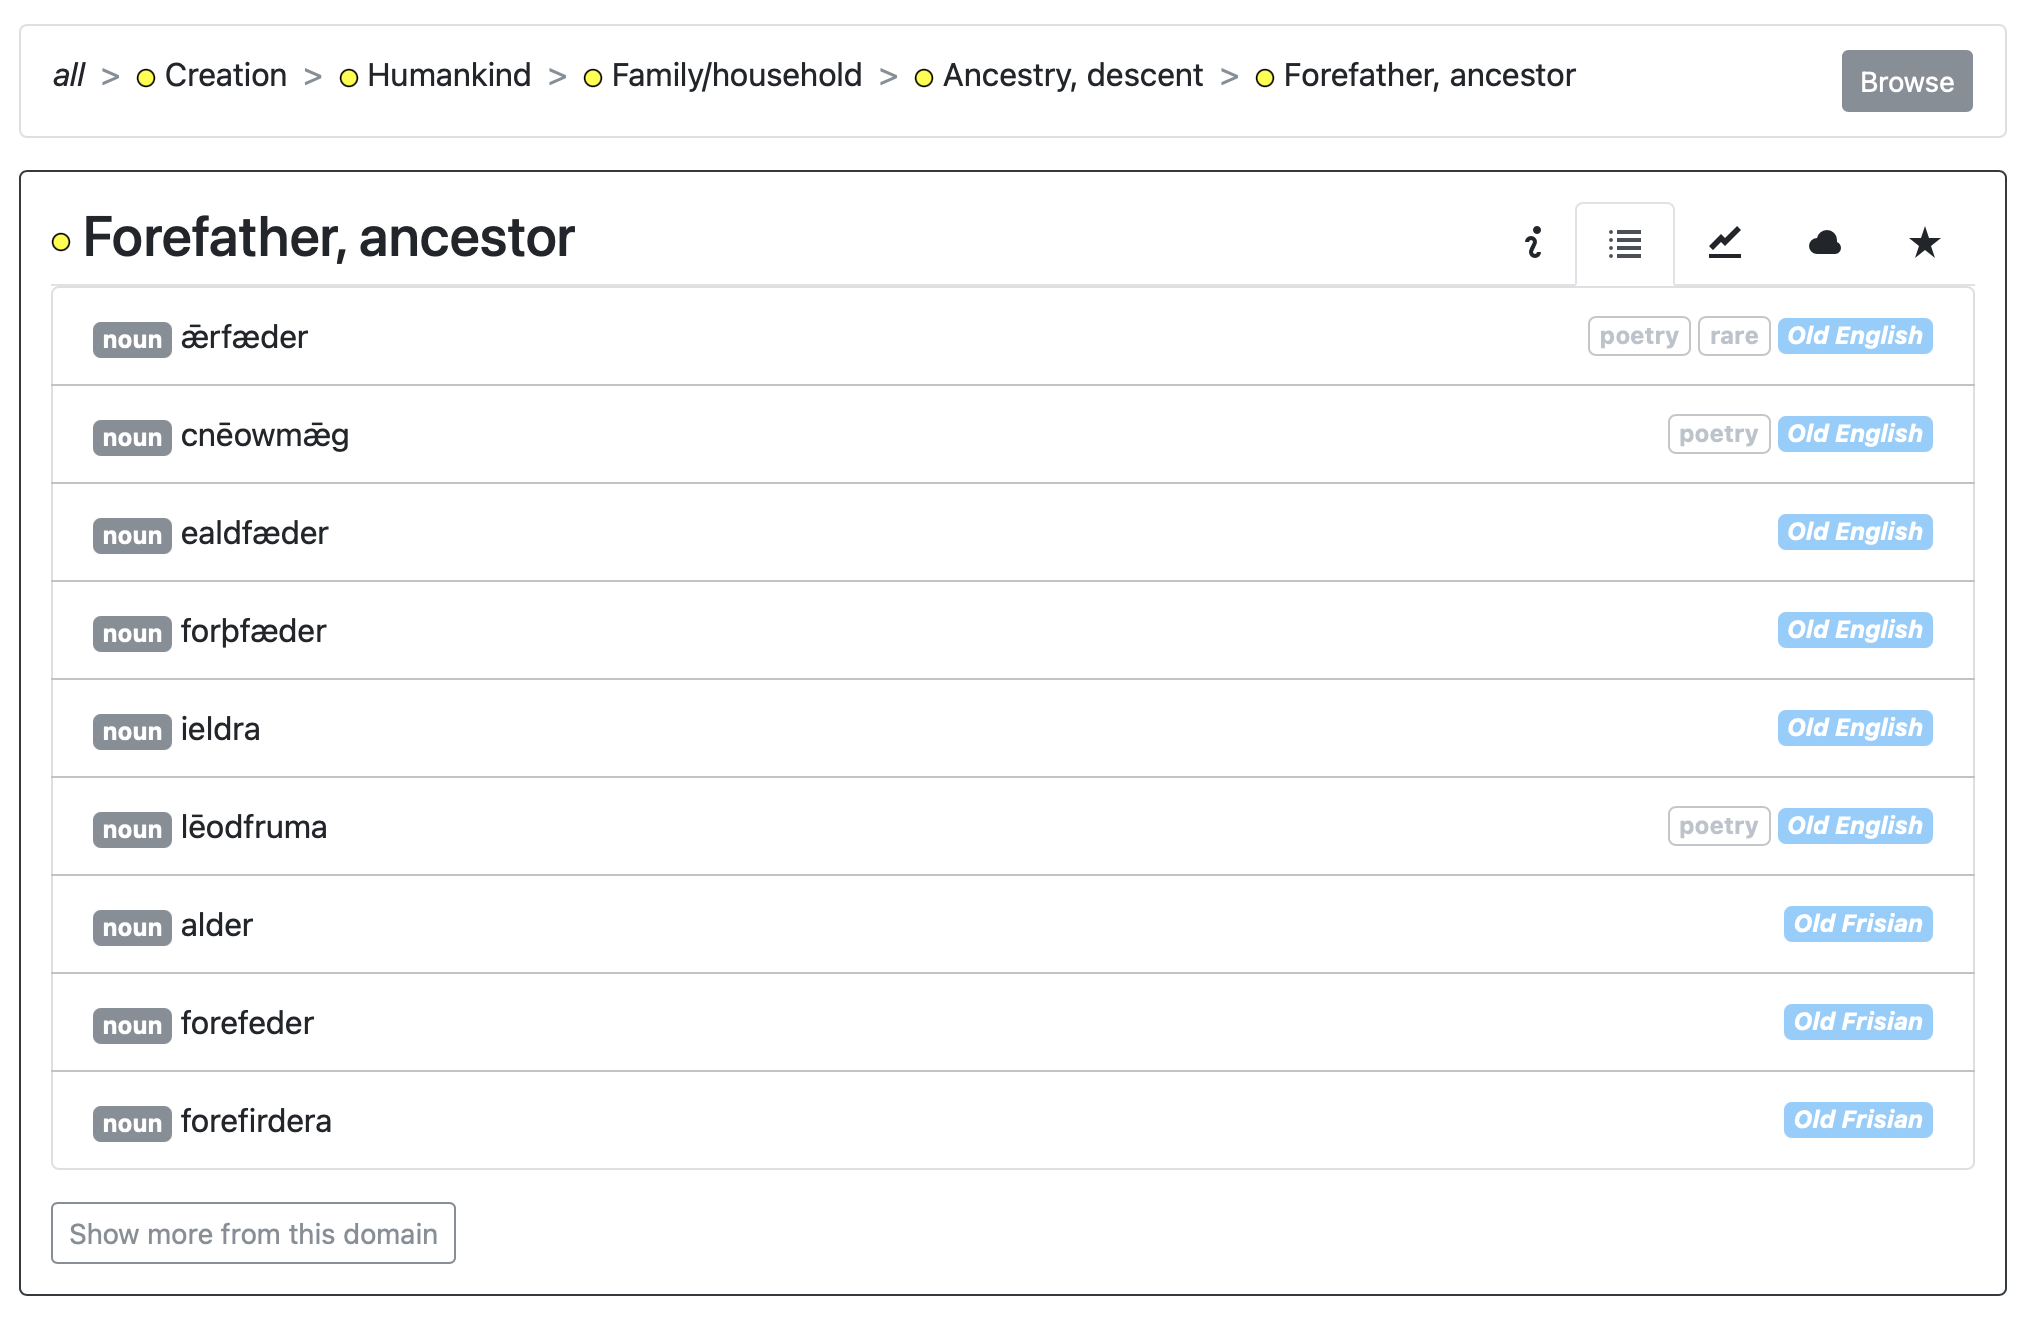
\includegraphics[width=\textwidth]{Stolk2021b/fig/Fig2.png}
	\caption[]{\label{fig:Stolk2021b:Fig2} List in Evoke of Old English and Old Frisian words denoting “02.03.02.03.03 Forefather, ancestor”.}
\end{figure}

The integration of Old Frisian and Old English into Evoke facilitates the comparison of the relationship between the lexicons of both languages. Cognates are words within the same language or in different languages that have a common etymological origin, and therefore resemble each other to a greater or lesser extent in form (Schmitt, 1997: 209; Otwinowska-Kasztelanic, 2011: 4). Awareness of cognates enhances the ability to learn another language — in this case, learning Old Frisian will be easier for someone who is familiar with Old English, and vice versa (Schmitt, 1997: 209; Otwinowska-Kasztelanic, 2011: 4-5).  Additionally, finding cognate words in a set of languages is the first step in the comparative method for historical linguists, allowing them to study the development of languages and the reconstruction of common ancestors (Baldi, 2011: 1-16; Trask, 2015: 198-233). Fig. \ref{fig:Stolk2021b:Fig3} lists the various synonyms (in Old English as well as Old Frisian) for Old English ealda fæder. Here, Old Frisian aldafeder is a cognate of the Old English word that is closest in form: ealda fæder. Similarities such as these, i.e. in both form and meaning, facilitate detection of cognates.

\begin{figure}[htbp]
	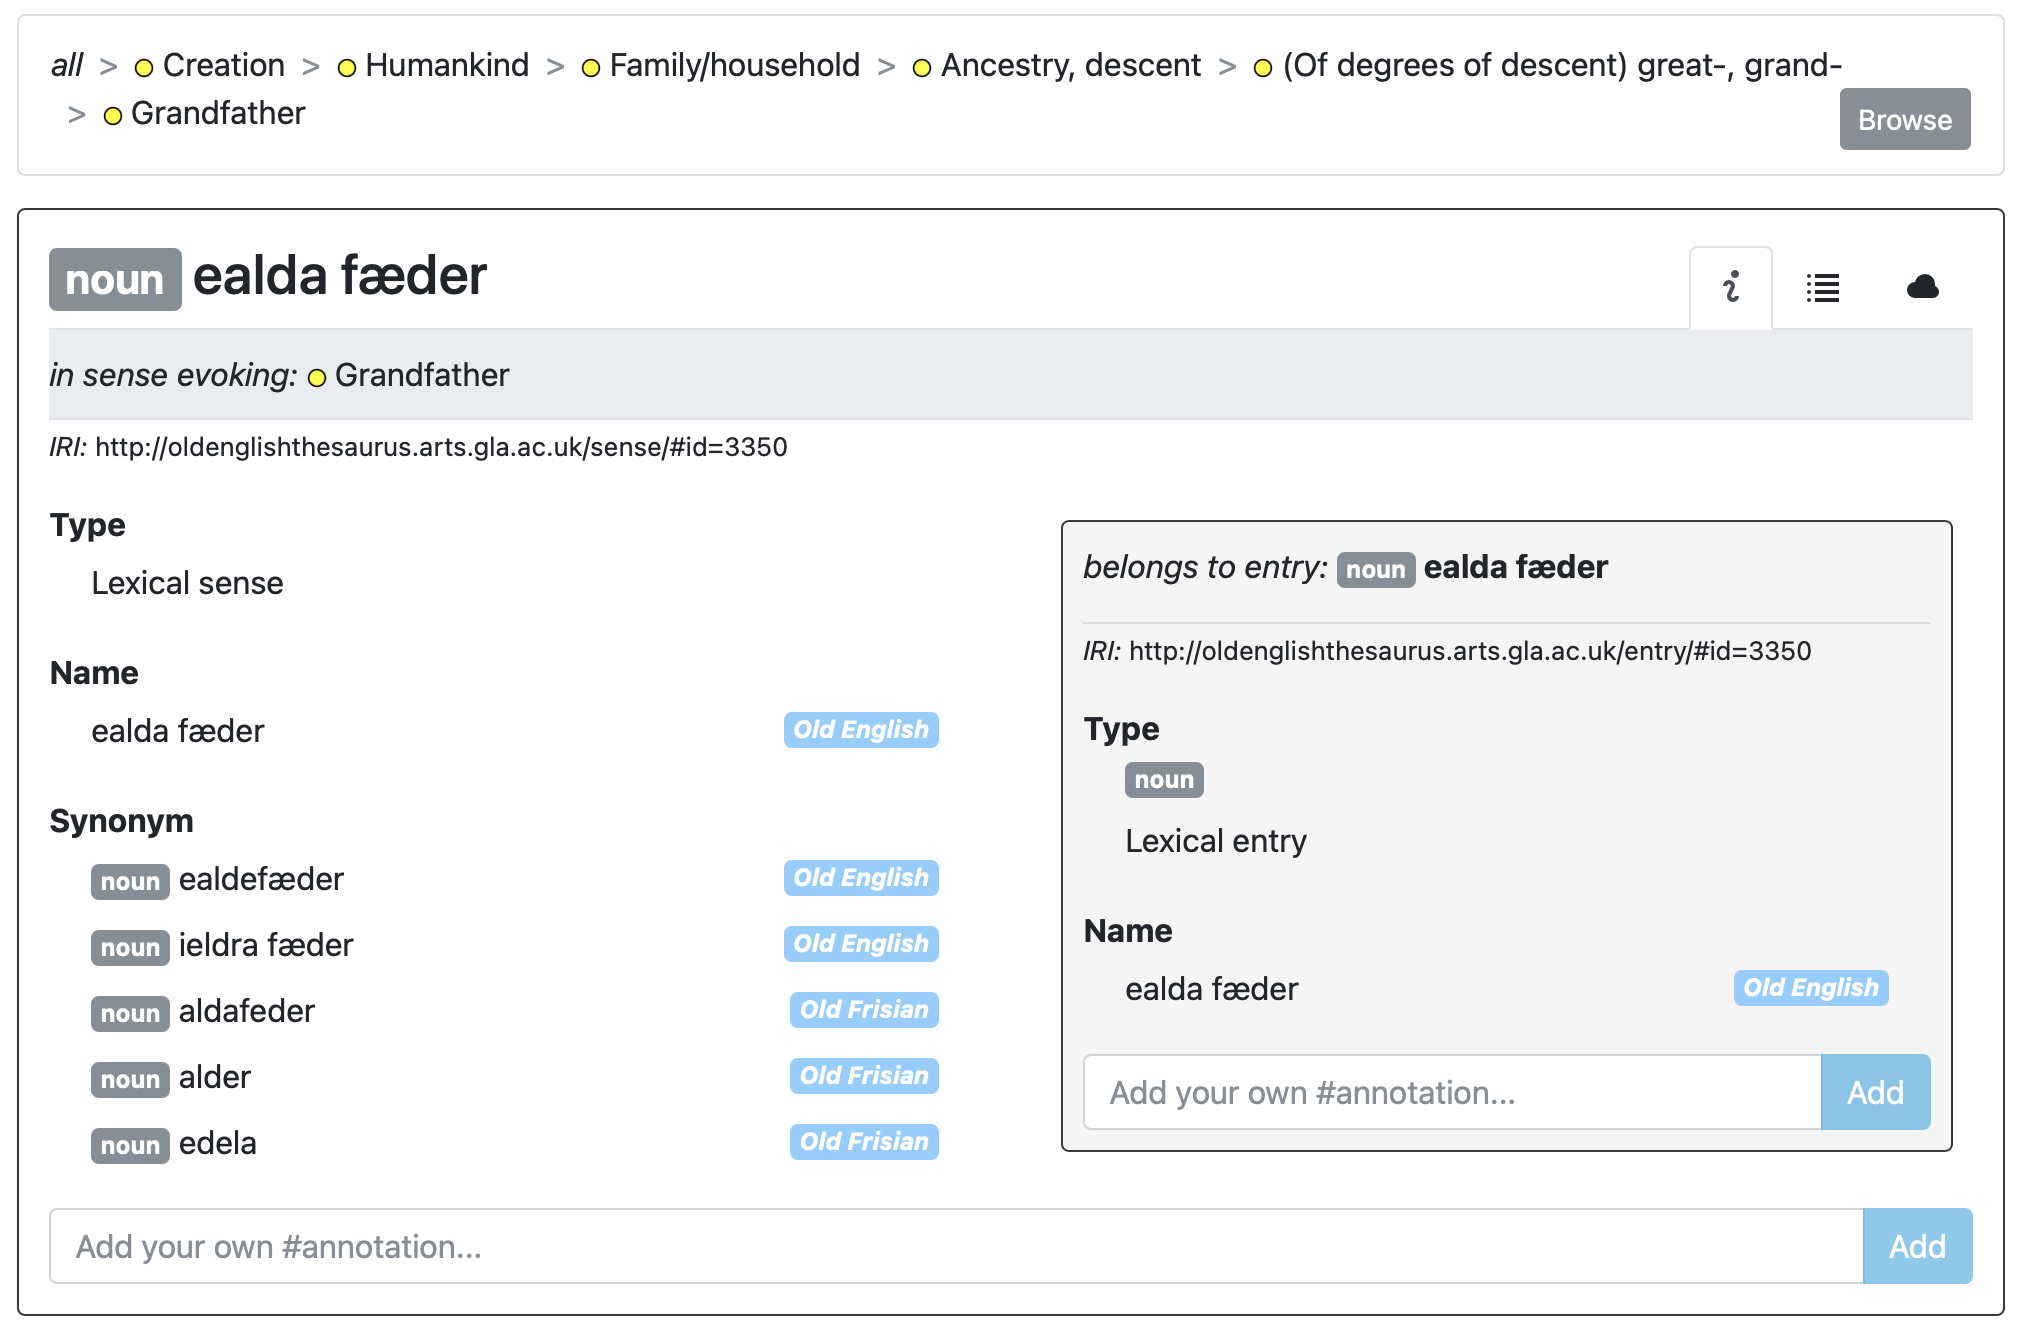
\includegraphics[width=\textwidth]{Stolk2021b/fig/Fig3.png}
	\caption[]{\label{fig:Stolk2021b:Fig3} Information in Evoke on Old English ealda fæder in the sense of “02.03.02.03.04 | 01 Grandfather”.}
\end{figure}

\subsection{\textsc{kinship} Terminology: Cultural Lexical Research of Cognates}
Onomasiological ordering of lexis can be useful for cultural lexical research. \textsc{kinship} terms are “ways in which people classify their kinship universe” and as such provide clues to the nature of a kinship system in a society as well as to the social statuses and roles of kinsmen (Fox, 1984: 243). Similar cultures often have very similar reference terms for relatives. It would go beyond the scope of this article to perform an entire analysis of the semantic field in question. However, to illustrate the usefulness of Evoke in comparing Old Frisian and Old English we undertake an exploratory comparative study of cosanguineal \textsc{kinship} terms. We have taken inspiration from well-known research by Lancaster on kinship terminology (1958). Her kinship tree graph, which contains cosanguineal nomenclature in Old English, has been expanded here with corresponding Old Frisian lexis (see Fig. \ref{fig:Stolk2021b:Fig4}). The graph, using a genealogical structure, contains nodes and lines to indicate individuals and relations of descent, respectively.  For every node in the graph, Evoke has been employed to locate the corresponding Old English and Old Frisian words. The results are shown in Table 2. 


\begin{figure}[htbp]
    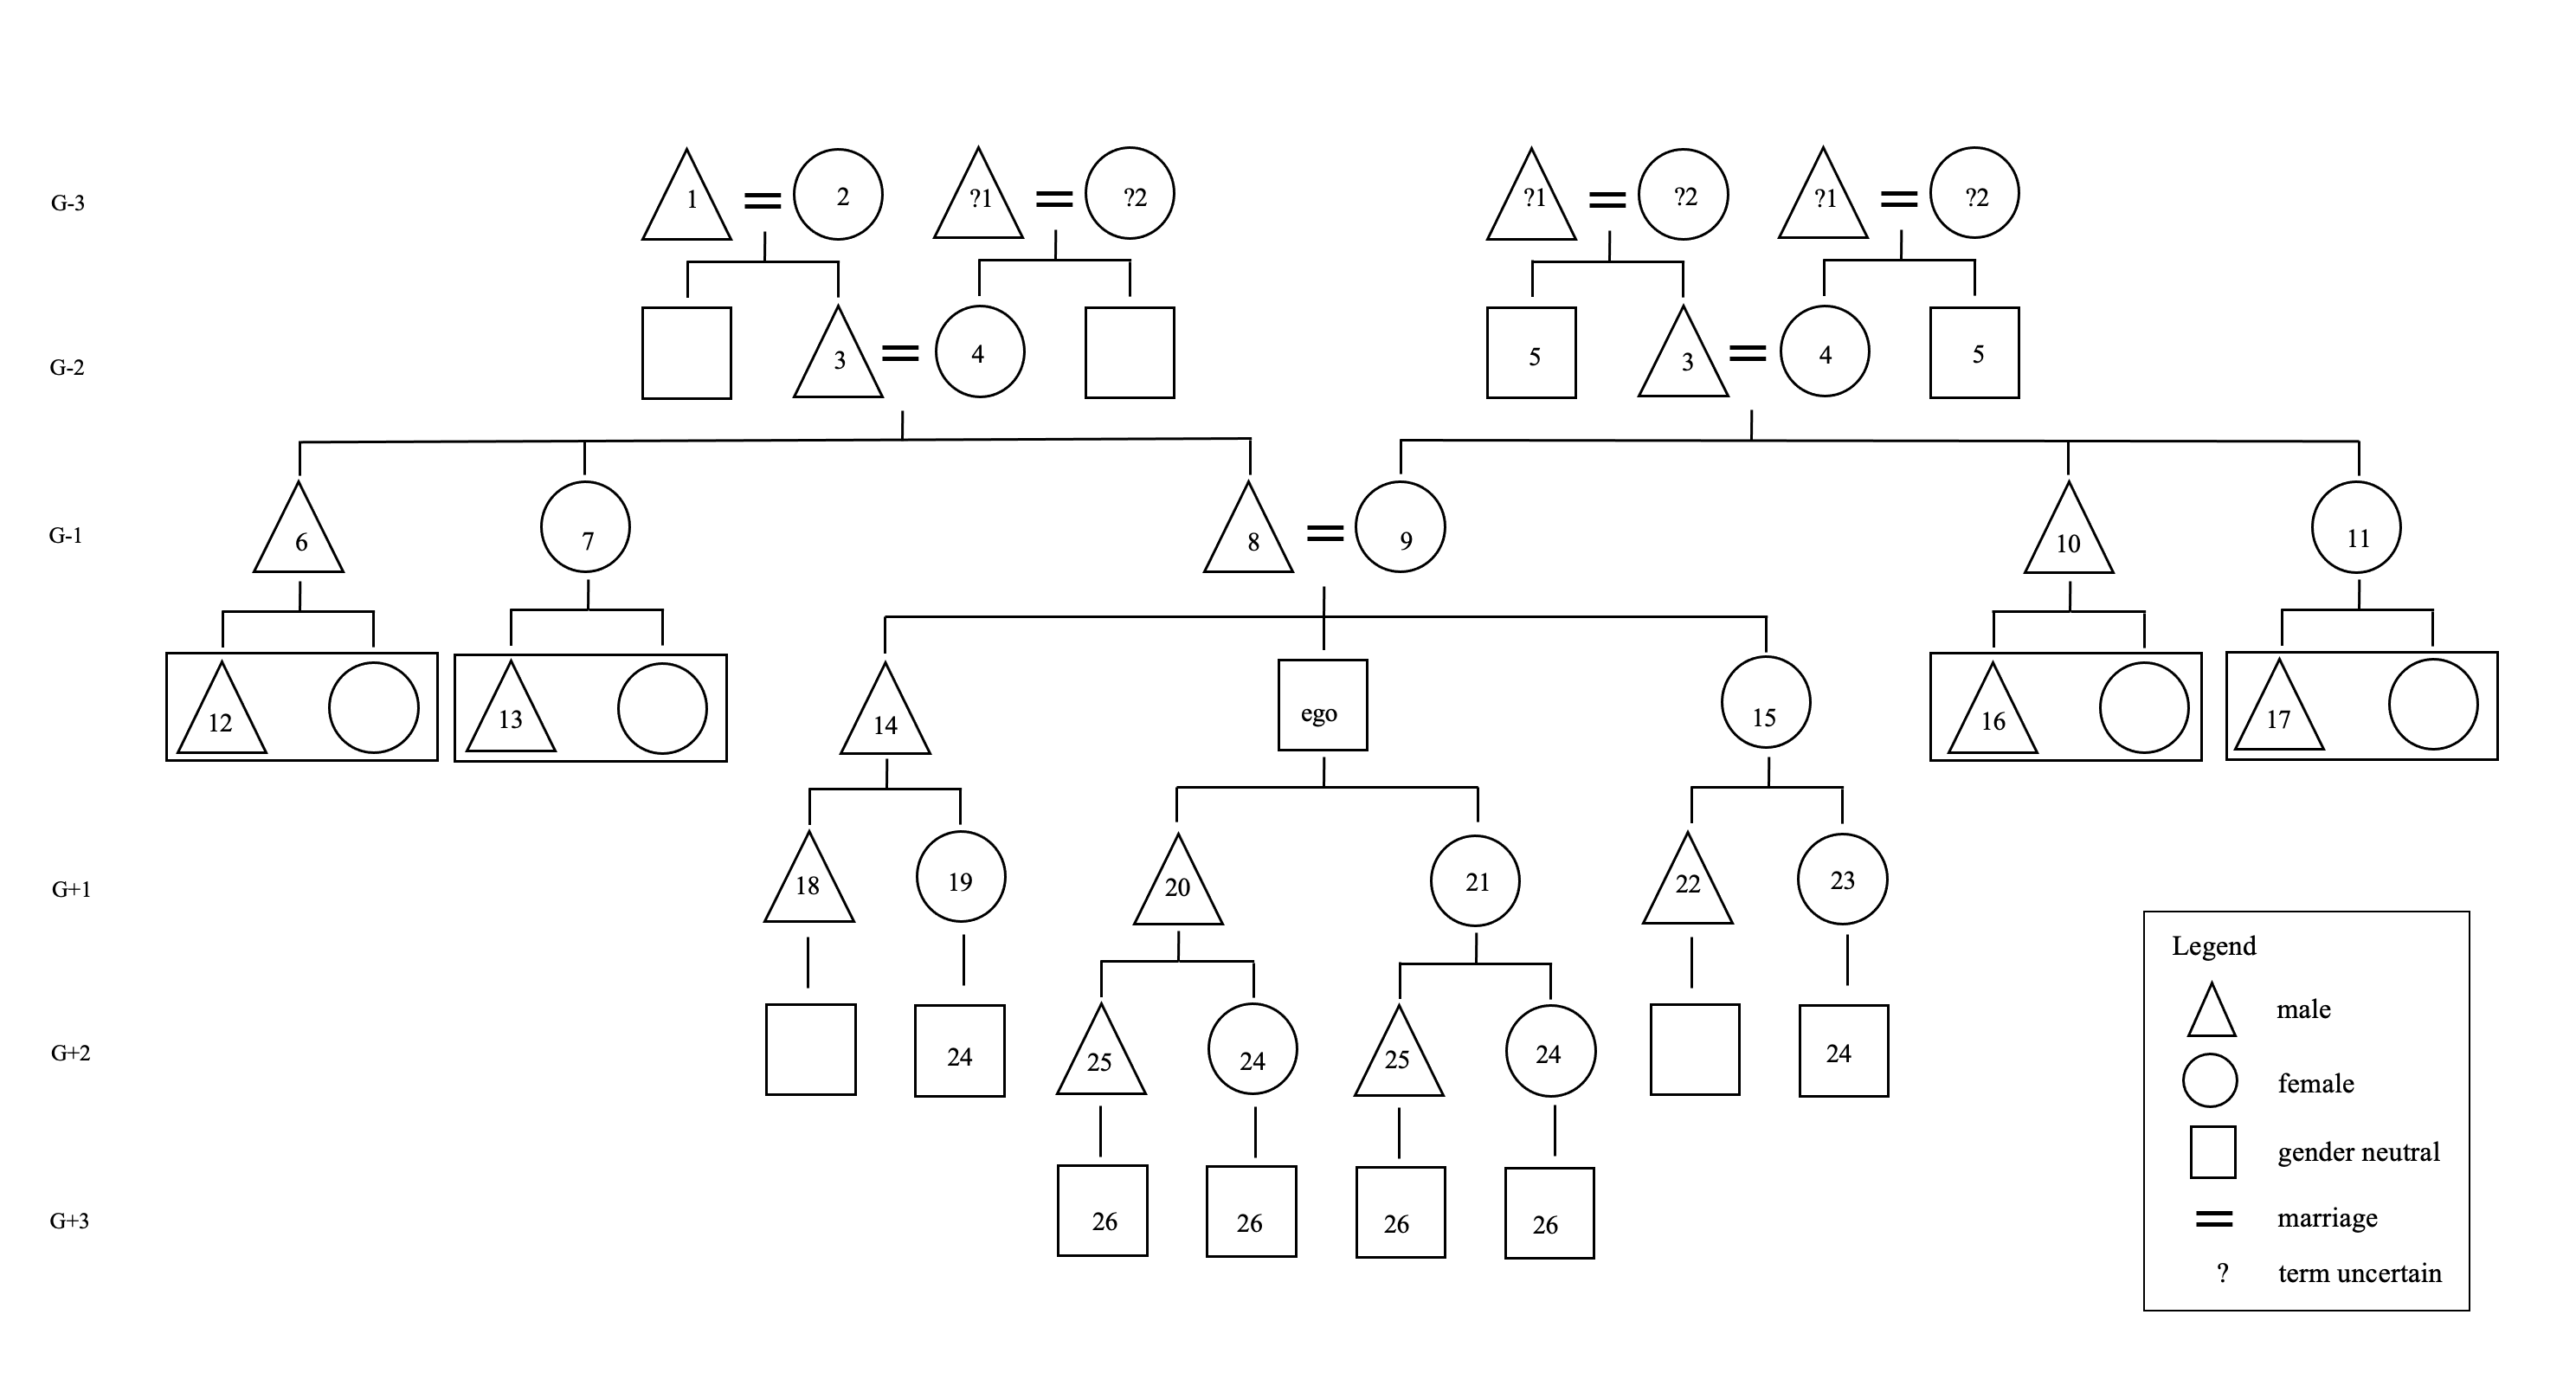
\includegraphics[width=\textwidth]{Stolk2021b/fig/Fig4.png}
	\caption[]{\label{fig:Stolk2021b:Fig4} Kinship relations.}
\end{figure}

No.	Old English	Old Frisian	Modern English
1	ieldra fæder, thridda fæder	edela, ūraldafeder, alder	great-grandfather
2	thridde mōdor	eldramōder, ūraldemōder	great-grandmother
3	ealde mōdor	aldemōder	grandmother
4	ealdafæder, ieldra fæder, ealda fæder	aldafeder, edela, alder	grandfather
5		aldaēm	granduncle
6	fædera	federia, federesbrōther	uncle, father's brother
7	fathu	fethu, federswester	aunt, father's sister
8	fæder	feder	father
9	mōdor, ācennicge, bearncennicge, cennestre, byrthe	mōder	mother
10	ēam	ēm, mōderesbrōther	uncle, mother's brother
11	mōdri(g)e	mōdire, mōie	aunt, mother's sister
12	mōdri(ge), (ge)swēor, geswigra	federiasune 	male cousin 
(father's brother's son)
13	fathusunu
mōdri(ge), (ge)swēor, geswigra	fethansune	male cousin 
(father's sister's son)
14	brōthor	brōther	brother
15	sweostor	swester	sister
16		emka, emessune	male cousin 
(mother's brother's son)
17		mōdiransune	male cousin 
(mother's sister's son)
18	(ge)nefa, brōthorsunu, suhterga	neva, brōthersune, 
brōtherbern, brōtherskind, swesternabern	nephew
19	nefene, nift, brōthordohtor	nifte, nifke, brōtheresdochter, 
brōtherbern, brōtherskind, swesternabern	niece
20	sunu, bearn, 
byrdling, byre, tūdor, eafora, geēacnung 	sune, bern, 
kind	son, child (general term)
21	dohtor, bearn, 
byrdling, byre, tūdor, eafora, geēacnung	dochter, bern, 
kind	daughter, child (general term)
22	(ge)nefa, sweostersunu, 
sweosterbearn	neva, swestersune, 
swester(na)bern, swesterkind, swesterling	nephew
23	nefene, nift, 
sweosterbearn	nifte, nifke, swesterdochter, 
swester(na)bern, swesterkind, swesterling	niece
24		niftlīn, niftakind	niece's child
25	grandson: sunsunu, nefa
granddaughter: nefe, nift	bernesbern, kindeskind	grandchild
26	great granddaughter: thridde dohtor
great grandson: thridda sunu	kindeskindeskind	great-grandchild
Table 2. Cosanguineal kinship terms in Old English and Old Frisian.

Comparison of the \textsc{kinship} terminology clearly demonstrates the close relationship between Old English and Old Frisian: cognate forms for similar terms in Table 2 are underlined. Old English and Old Frisian have cognates for the lexis for: father (Fa), mother (Mo), brother (Br), sister (Si), son (So), daughter (Da), child, grandfather, grandmother, maternal uncle (MoBr) and aunt (MoSi), paternal uncle (FaBr) and aunt (FaSi), nephew and niece. Terms for some other bloodrelations likewise show similar cognate (compound) forms, i.e. great grandfather, greatgrandmother, cousins.

Old Frisian possessed terms for kinship relations that are not found in Old English: mōdiransune, emessune, aldaēm. When no Old English lexeme is recorded for a specific sense, it should not be inferred that the concept as such was absent in Old English. Notions such as “father’s brother’s son” and “mother’s sister’s son” exist in Old English, but are not lexicalized. Instead, they were expressed with genitival phrases (fæderan sunu and modiran sunu).

\section{Analysis}
\label{sect:Stolk2021b:Analysis}

Based on the data from TOE and the newly created dataset, this section presents a detailed analysis of both the Old English and the Old Frisian lexis located under the semantic field of “02.03.02 Family/household” through the use of the web application Evoke. Evoke offers quantitative information from TOE, possibly in combination with additional datasets, in two forms: (1) basic statistics for a specific category and (2) advanced statistics that incorporate the onomasiological structure of TOE more fully, which also allow for queries to be customized. 

\subsection{Analysis of Parts of Speech Distribution}
The basic statistics of Evoke allow us to provide some insight into matters such as the distribution of the parts of speech within the semantic field of \textsc{kinship}, represented by the TOE category “02.03.02 Family/household” and all its subordinate categories. Fig. \ref{fig:Stolk2021b:Fig5} shows the distributions for Old English senses and of Old Frisian ones. When contrasting these figures, the percentages of nouns for Old English and Old Frisian turn out to be comparable. However, Old Frisian has relatively fewer adjectives and more verbs, adverbs, and phrases than Old English. The marked difference between the relative number of verbs and that of adjectives is especially striking and merits further research.

\begin{figure}[htbp]
	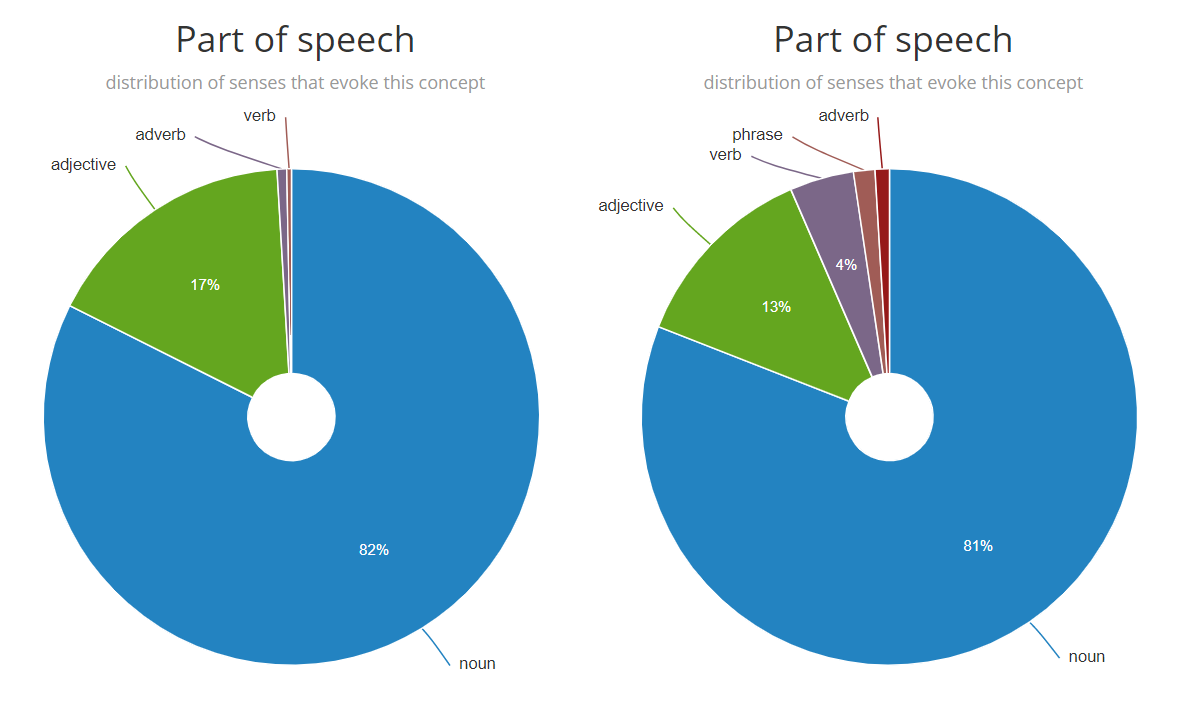
\includegraphics[width=\textwidth]{Stolk2021b/fig/Fig5.png}
	\caption[]{\label{fig:Stolk2021b:Fig5} Distribution of Old English (left) and Old Frisian (right) senses in “02.03.02 Family/household”.}
\end{figure}


\subsection{Degree of Polysemy}
The advanced statistics section of Evoke renders, amongst others, a graph that indicates polysemy: the number of senses attributed to a lemma. Indeed, polysemy (and homonymy) can be a measure of the ambiguity of words, demanding the interpreting party to reflect carefully on the intended meaning in an utterance (Chandler and Munday, 2016: s.v. polysemy). Fig. \ref{fig:Stolk2021b:Fig6} demonstrates that, within the taxonomy branch of “02.03.02 Family/household”, the vast majority of Old Frisian lemmata is monosemous (i.e., 90\% has a single recorded sense), whereas Old English has, relatively speaking, more lemmata that are polysemous. This outcome can partially be explained by the fact that AFWB, which was used to obtain the Old Frisian lemmata and senses, is a concise dictionary and therefore does not record senses extensively. Even so, AFWB records multiple senses for entries when these senses are distinct enough to be necessary for initial readings of Old Frisian texts. The lack of polysemy for Old Frisian is striking, even when the nature of the source dictionary is taken into account. Whether this finding is characteristic of the language itself remains as yet undecided. The apparent monosemous nature of Old Frisian may be due to the lack of register variety in the surviving corpus. The Old Frisian corpus is predominantly juridical in nature whereas the Old English one is much more balanced, containg samples of different style varieties and registers, resulting in a higher number of polysemous words. 


\begin{figure}[htbp]
	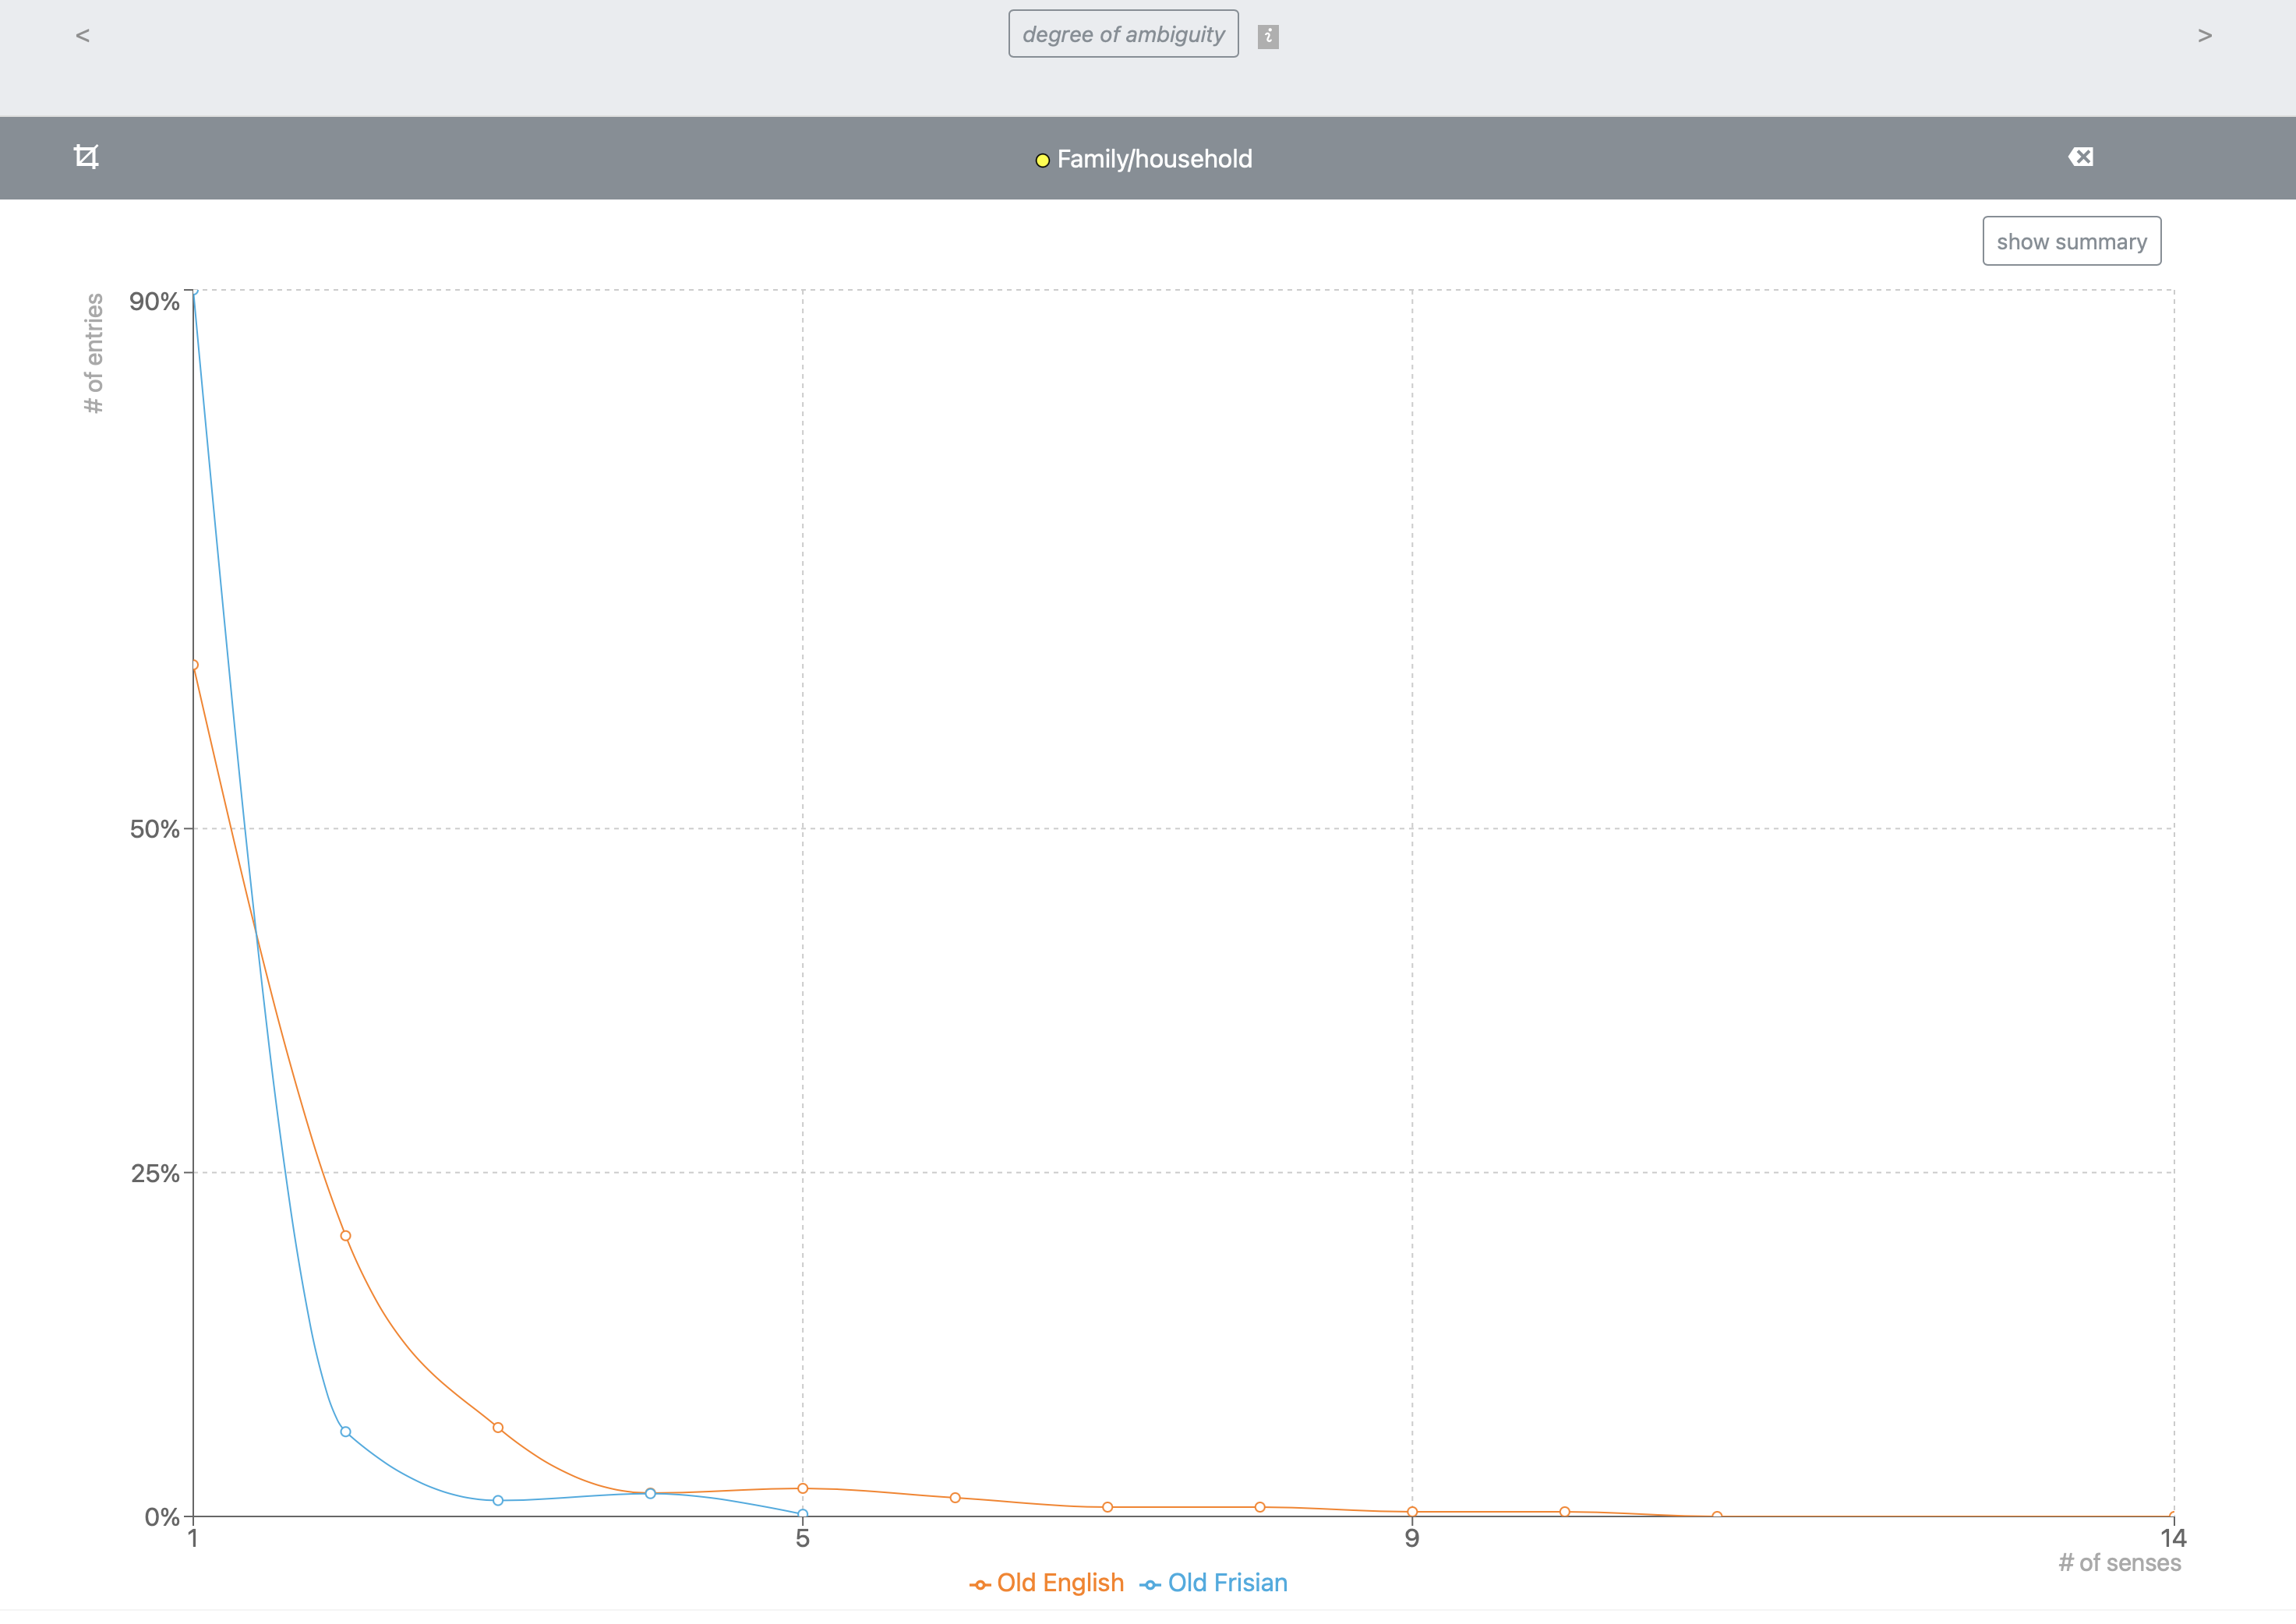
\includegraphics[width=\textwidth]{Stolk2021b/fig/Fig6.png}
	\caption[]{\label{fig:Stolk2021b:Fig6} Degree of polysemy within “02.03.02 Family/household”.}
\end{figure}


\subsection{Onomasiological Distribution over Taxonomy Levels}
Fig. \ref{fig:Stolk2021b:Fig7} shows the distribution of lexical senses over the various levels of the taxonomy, which is another advanced analysis offered by Evoke.  This diagram indicates that Old Frisian has more recorded senses located at taxonomy levels with highly specialized meanings than Old English (see levels 8–12). Moreover, Old Frisian features senses that are allocated to levels beyond those in use for Old English (levels 10–12). Indeed, many of the categories newly created for the purposes of capturing \textsc{kinship} in Old Frisian have been added as subordinate ones to TOE categories in the more specialized levels of the taxonomy. This diagram visualizes that outcome. A possible explanation may be that Old Frisian texts are mainly juridical in nature, very often pertaining to inheritance law, and therefore deal with more precise meanings that denote family relationships. A case in point is the degree of kinship, for which the Old Frisian lexis that has come down to us includes fine-grained senses (see also Table 2). 


\begin{figure}[htbp]
	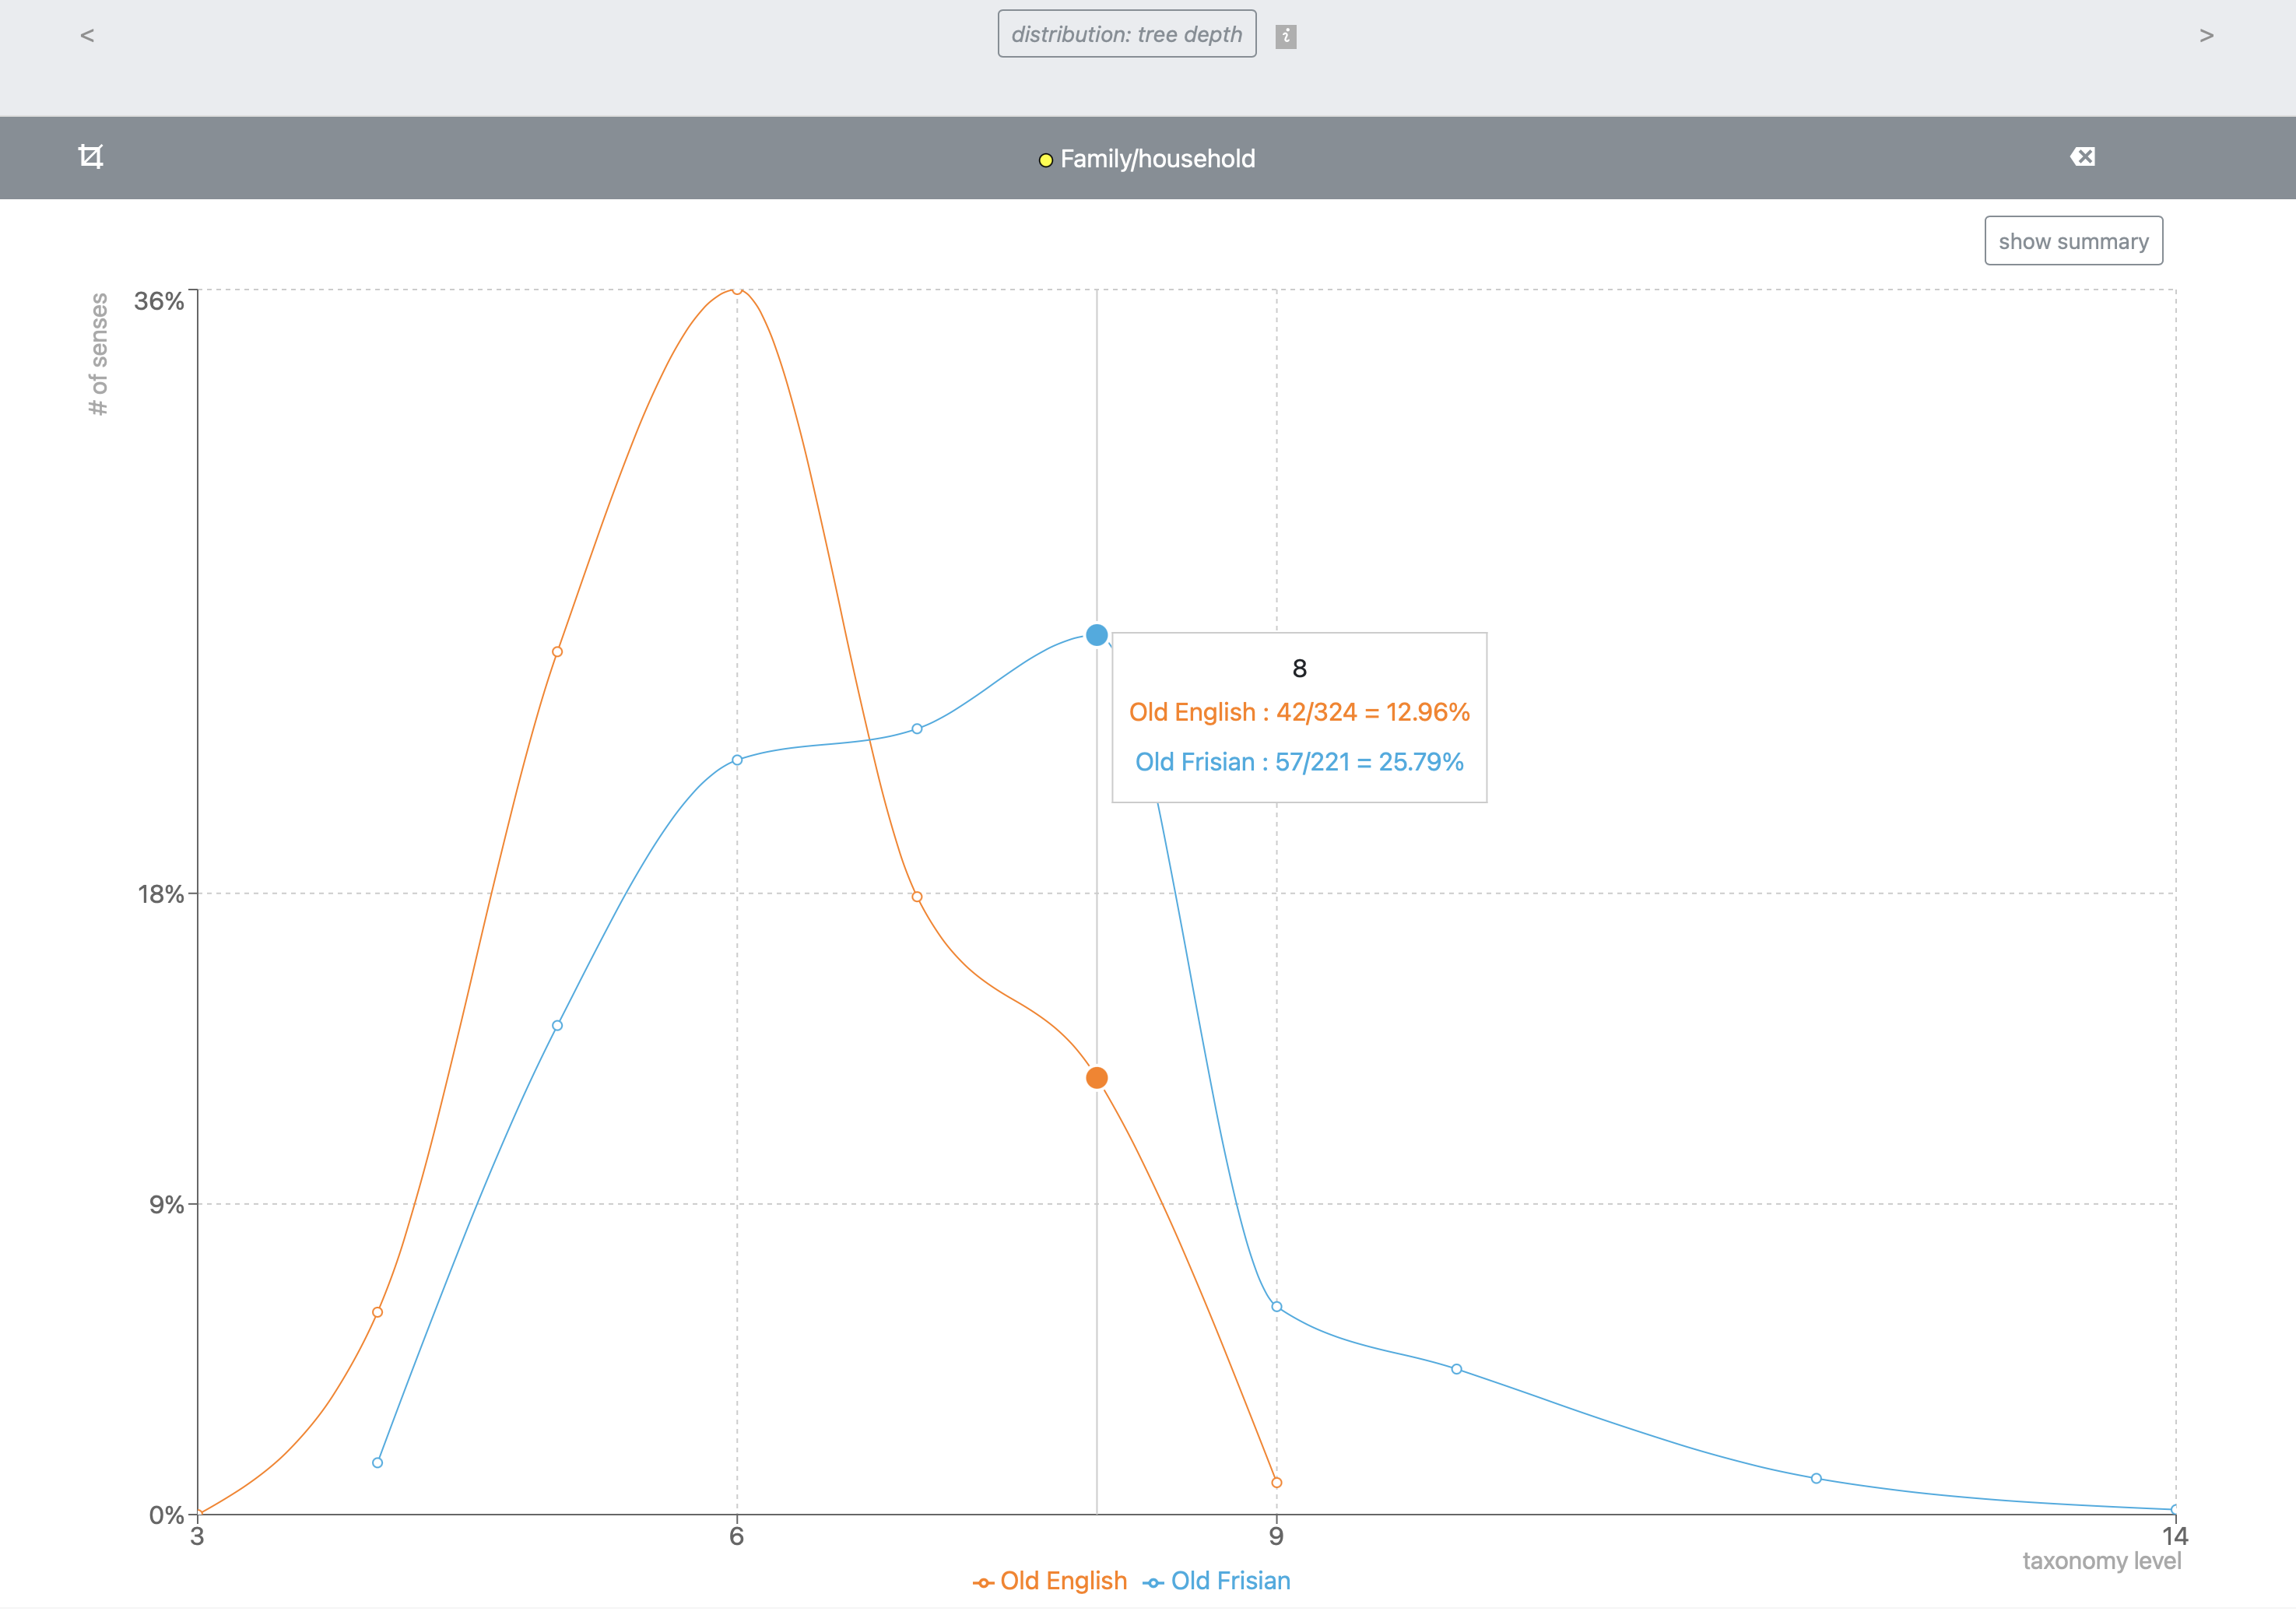
\includegraphics[width=\textwidth]{Stolk2021b/fig/Fig7.png}
	\caption[]{\label{fig:Stolk2021b:Fig7} Distribution of lexical senses within “02.03.02 Family/household” over the taxonomy levels.}
\end{figure}


\subsection{Onomasiological Distribution over Categories}
\label{sect:Stolk2021b:OnomasiologicalDistrubtionOverCategories}
Distributions over thesaurus categories yield data regarding the degrees of lexicalization (also known as cultural elaboration) of semantic fields, which enables comparisons between them (Wierzbicka, 1997: 10-11). Fig. \ref{fig:Stolk2021b:Fig8} charts such a distribution for the subcategories of “02.03.02 Family/household”, generated with the advanced statistics section of Evoke.  The Y-axis has been configured to show the relative number of senses from a single language (i.e. Old Frisian or Old English) found within each branch indicated on the X-axis. The branch “02.03.02.03 Ancestry, descent”, highlighted in the diagram, contains the vast majority of the Old Frisian senses on \textsc{kinship} (170 senses or 79\%). The majority of Old English senses is found in the same branch, albeit less dominant (61\%) in relation to the other branches within the field. In fact, “02.03.02.03 Ancestry, descent” is the sole branch for which Old Frisian has a higher relative number of senses recorded than Old English. All other branches – i.e. “02.03.02.04 Adoption”, “02.03.02.02 Child, offspring”, “02.03.02.01 Parent”, and “02.03.02.05 Spiritual relationships” – have more Old English senses recorded than Old Frisian ones both in absolute and in relative numbers. The most striking differences between the two languages on this level are, therefore, (1) the relative degrees of lexicalization of “02.03.02.03 Ancestry, descent” and (2) the lack of any recorded Old Frisian senses for the concept of “02.03.02.04 Adoption”. 

Apart from “02.03.02.04 Adoption”, the Old Frisian corpus does not contain words for a number of other concepts found in Old English. These concepts are, most notably, represented by the TOE categories of “02.03.02.04.01 Foster relationships”, “02.03.02.02 | 06.01 A foundling”, “02.03.02.02.01 Twins”, and “02.03.02.02.02 Triplets”.  \textsc{kinship} concepts that witness a larger degree of lexicalization in Old Frisian in comparison to Old English are those that have been newly introduced (see Appendix 2), of course. However, they also include concepts that are gender neutral (such as expressed with Old Frisian swesterne ‘sibling’, for which TOE records no Old English equivalent) and concepts represented in TOE by the categories “02.03.02.03.06.02.06 In-law relationships”, “02.03.02.03.06.02.03 Child of brother/sister”, “02.03.02.03.06.02.04 Cousin”, and “02.03.02.02.05 | 02 A Bastard”. 

\begin{figure}[htbp]
	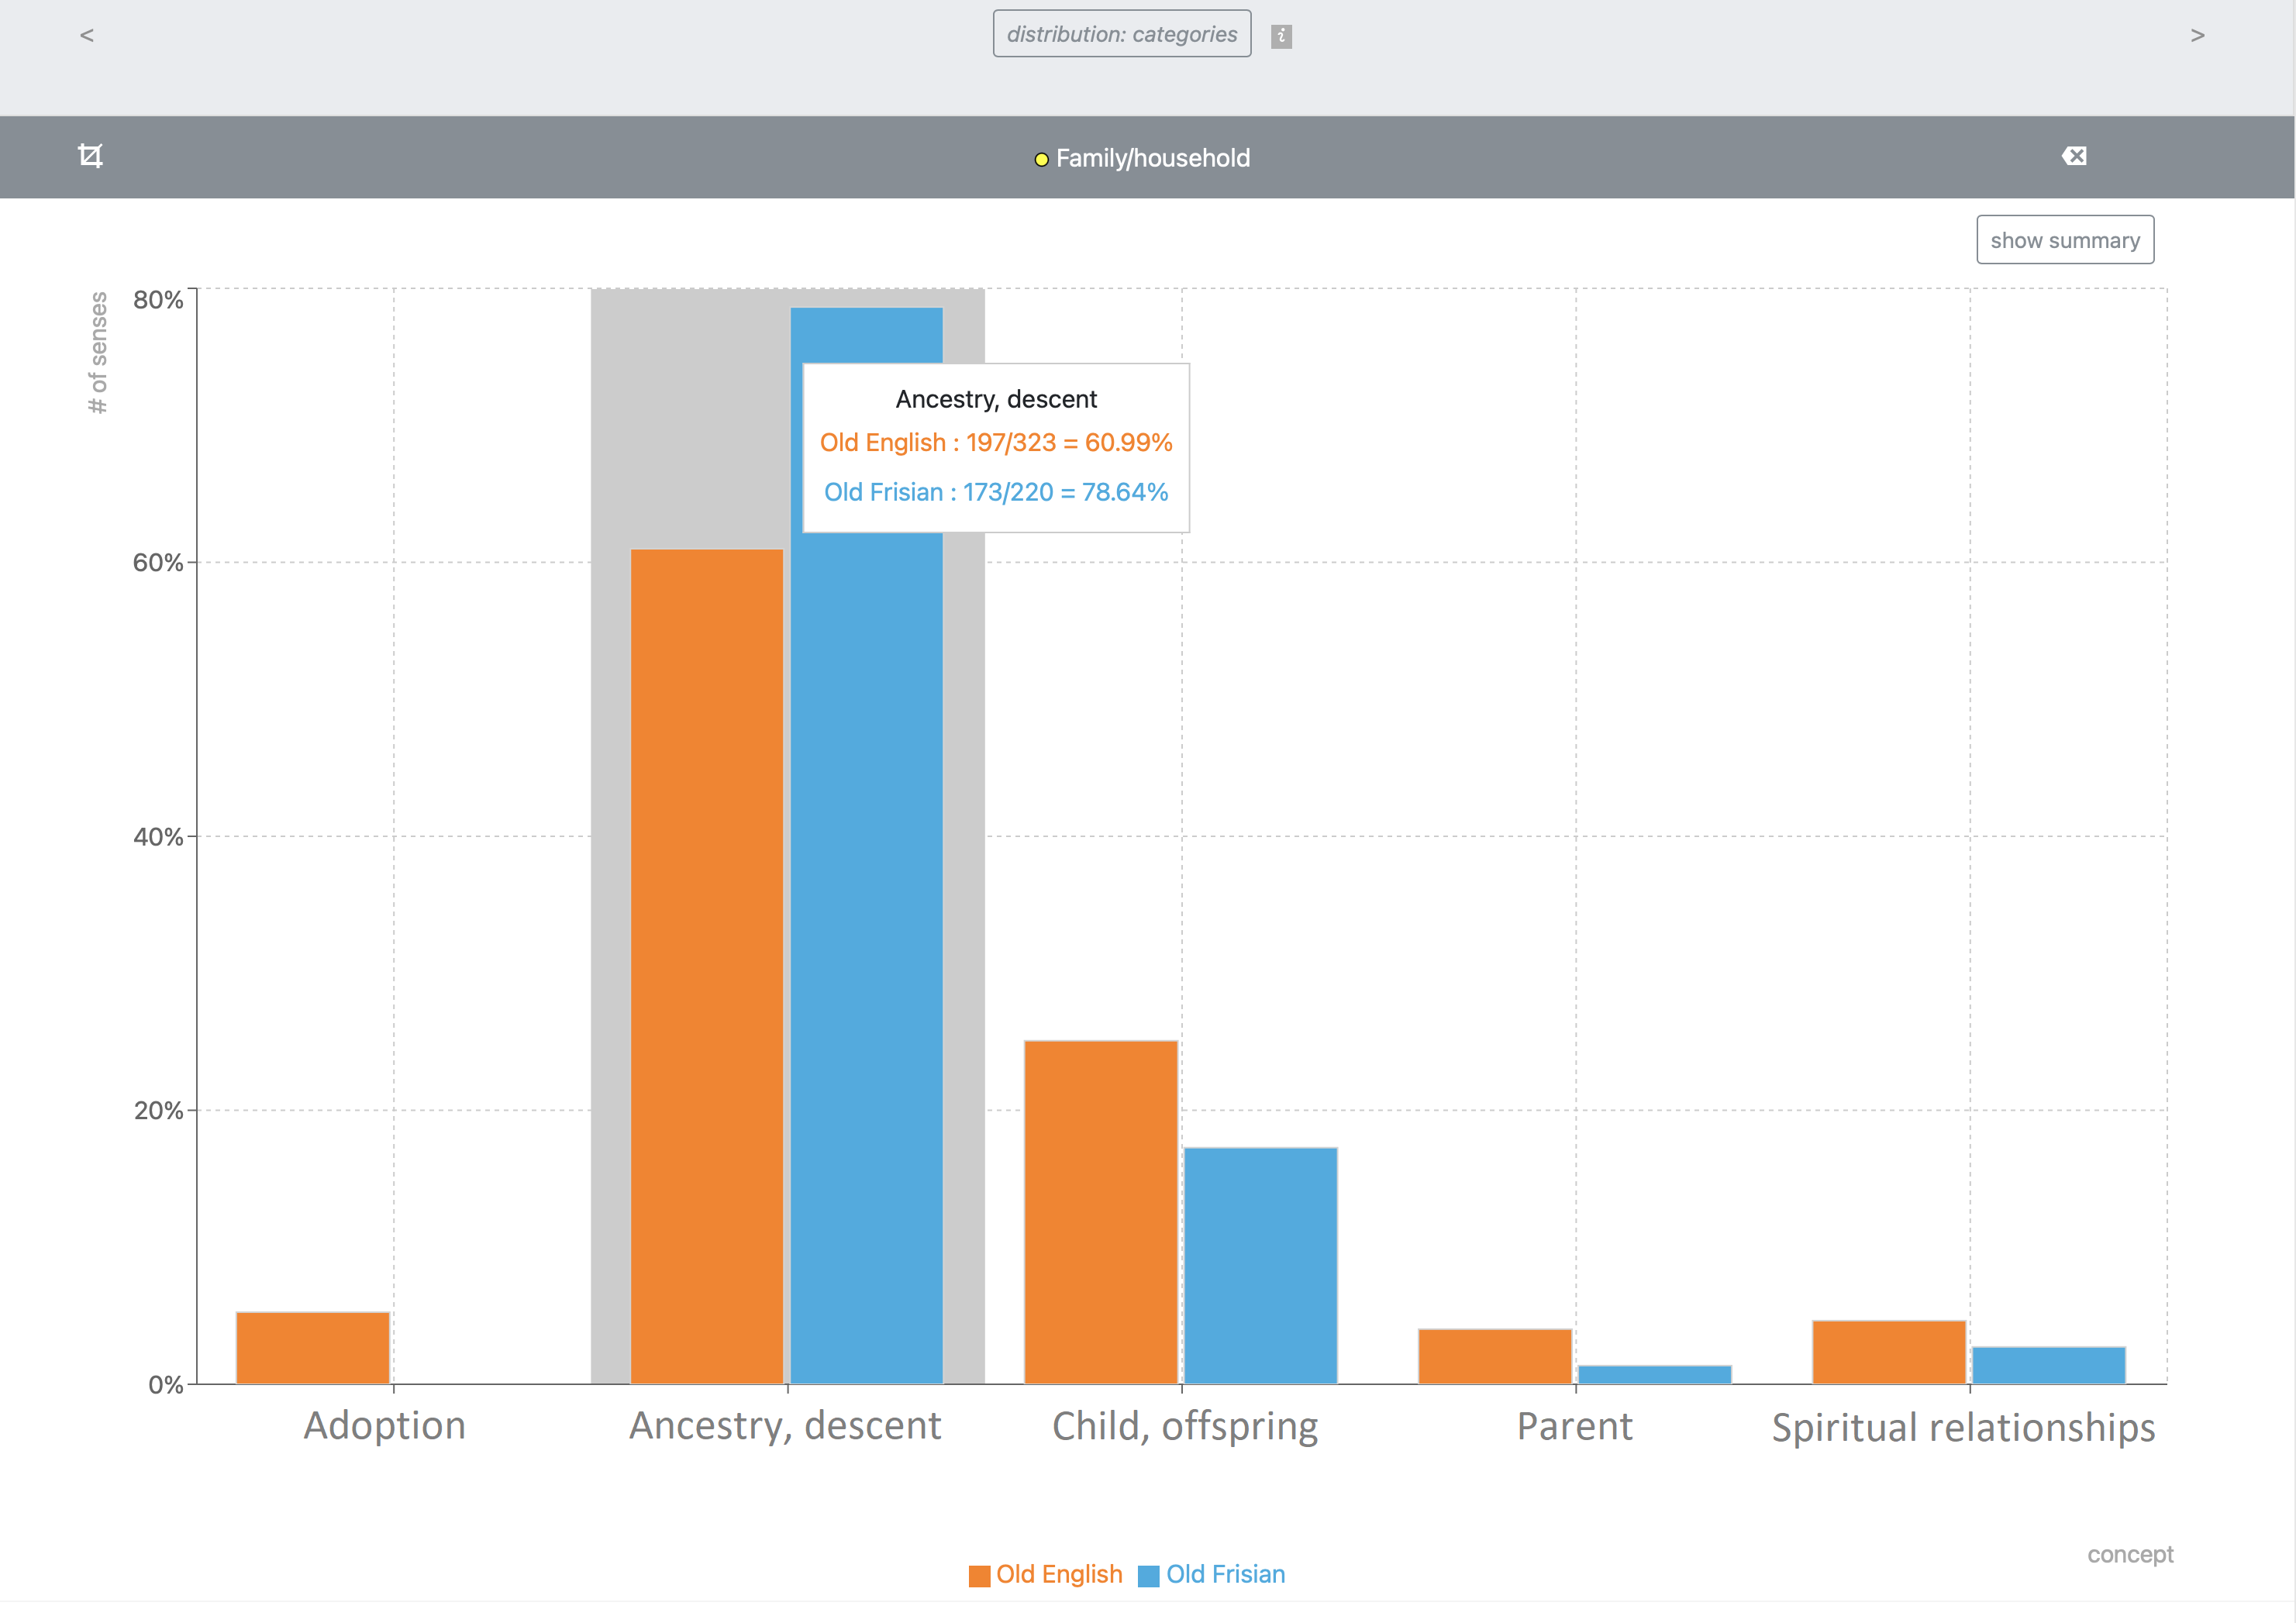
\includegraphics[width=\textwidth]{Stolk2021b/fig/Fig8.png}
	\caption[]{\label{fig:Stolk2021b:Fig8} Distribution of lexical senses over the semantic subfields of “02.03.02 Family/household”.}
\end{figure}


An extensive analysis of the distributions found in the more specific levels of the taxonomy branches is beyond the scope of this article. Nevertheless, to show what results such an analysis may produce, we include some insights into one such distribution here. Fig. \ref{fig:Stolk2021b:Fig9} presents the dispersion for “02.03.02.02.05 Having the same parents”, a subcategory of “02.03.02.02 Child, offspring”, which has a high degree of lexicalization for Old Frisian compared to Old English.  Some interesting observations can be made about this diagram: Old Frisian has more words than Old English with senses of “02.03.02.02.05.02 Sister” and “02.03.02.02.05 | 02 A Bastard”. The latter is even expressed with a word specific to a child born before its parents were married: spilkind. The category “02.03.02.02.05.03 Siblings” has been created for the Old Frisian lexis, since no Old English lexemes are recorded for this concept that leaves gender unspecified. The higher degree of lexicalization of both “02.03.02.02.05.02 Sister” and “02.03.02.02.05.03 Siblings” in Old Frisian compared to Old English, along with a lower degree for “02.03.02.02.05.01 Brother”, suggests that the level of expressivity for this kinship tie is more alike for members of the male and female sex in medieval Frisia than in the Anglo-Saxon kingdoms. Further research is warranted into the question whether this hypothesis will hold when these semantic fields are compared for attestation of lexis in solely juridical texts, which constitute the majority of the surviving Old Frisian written legacy but only a fraction of the much vaster Old English corpus.


\begin{figure}[htbp]
	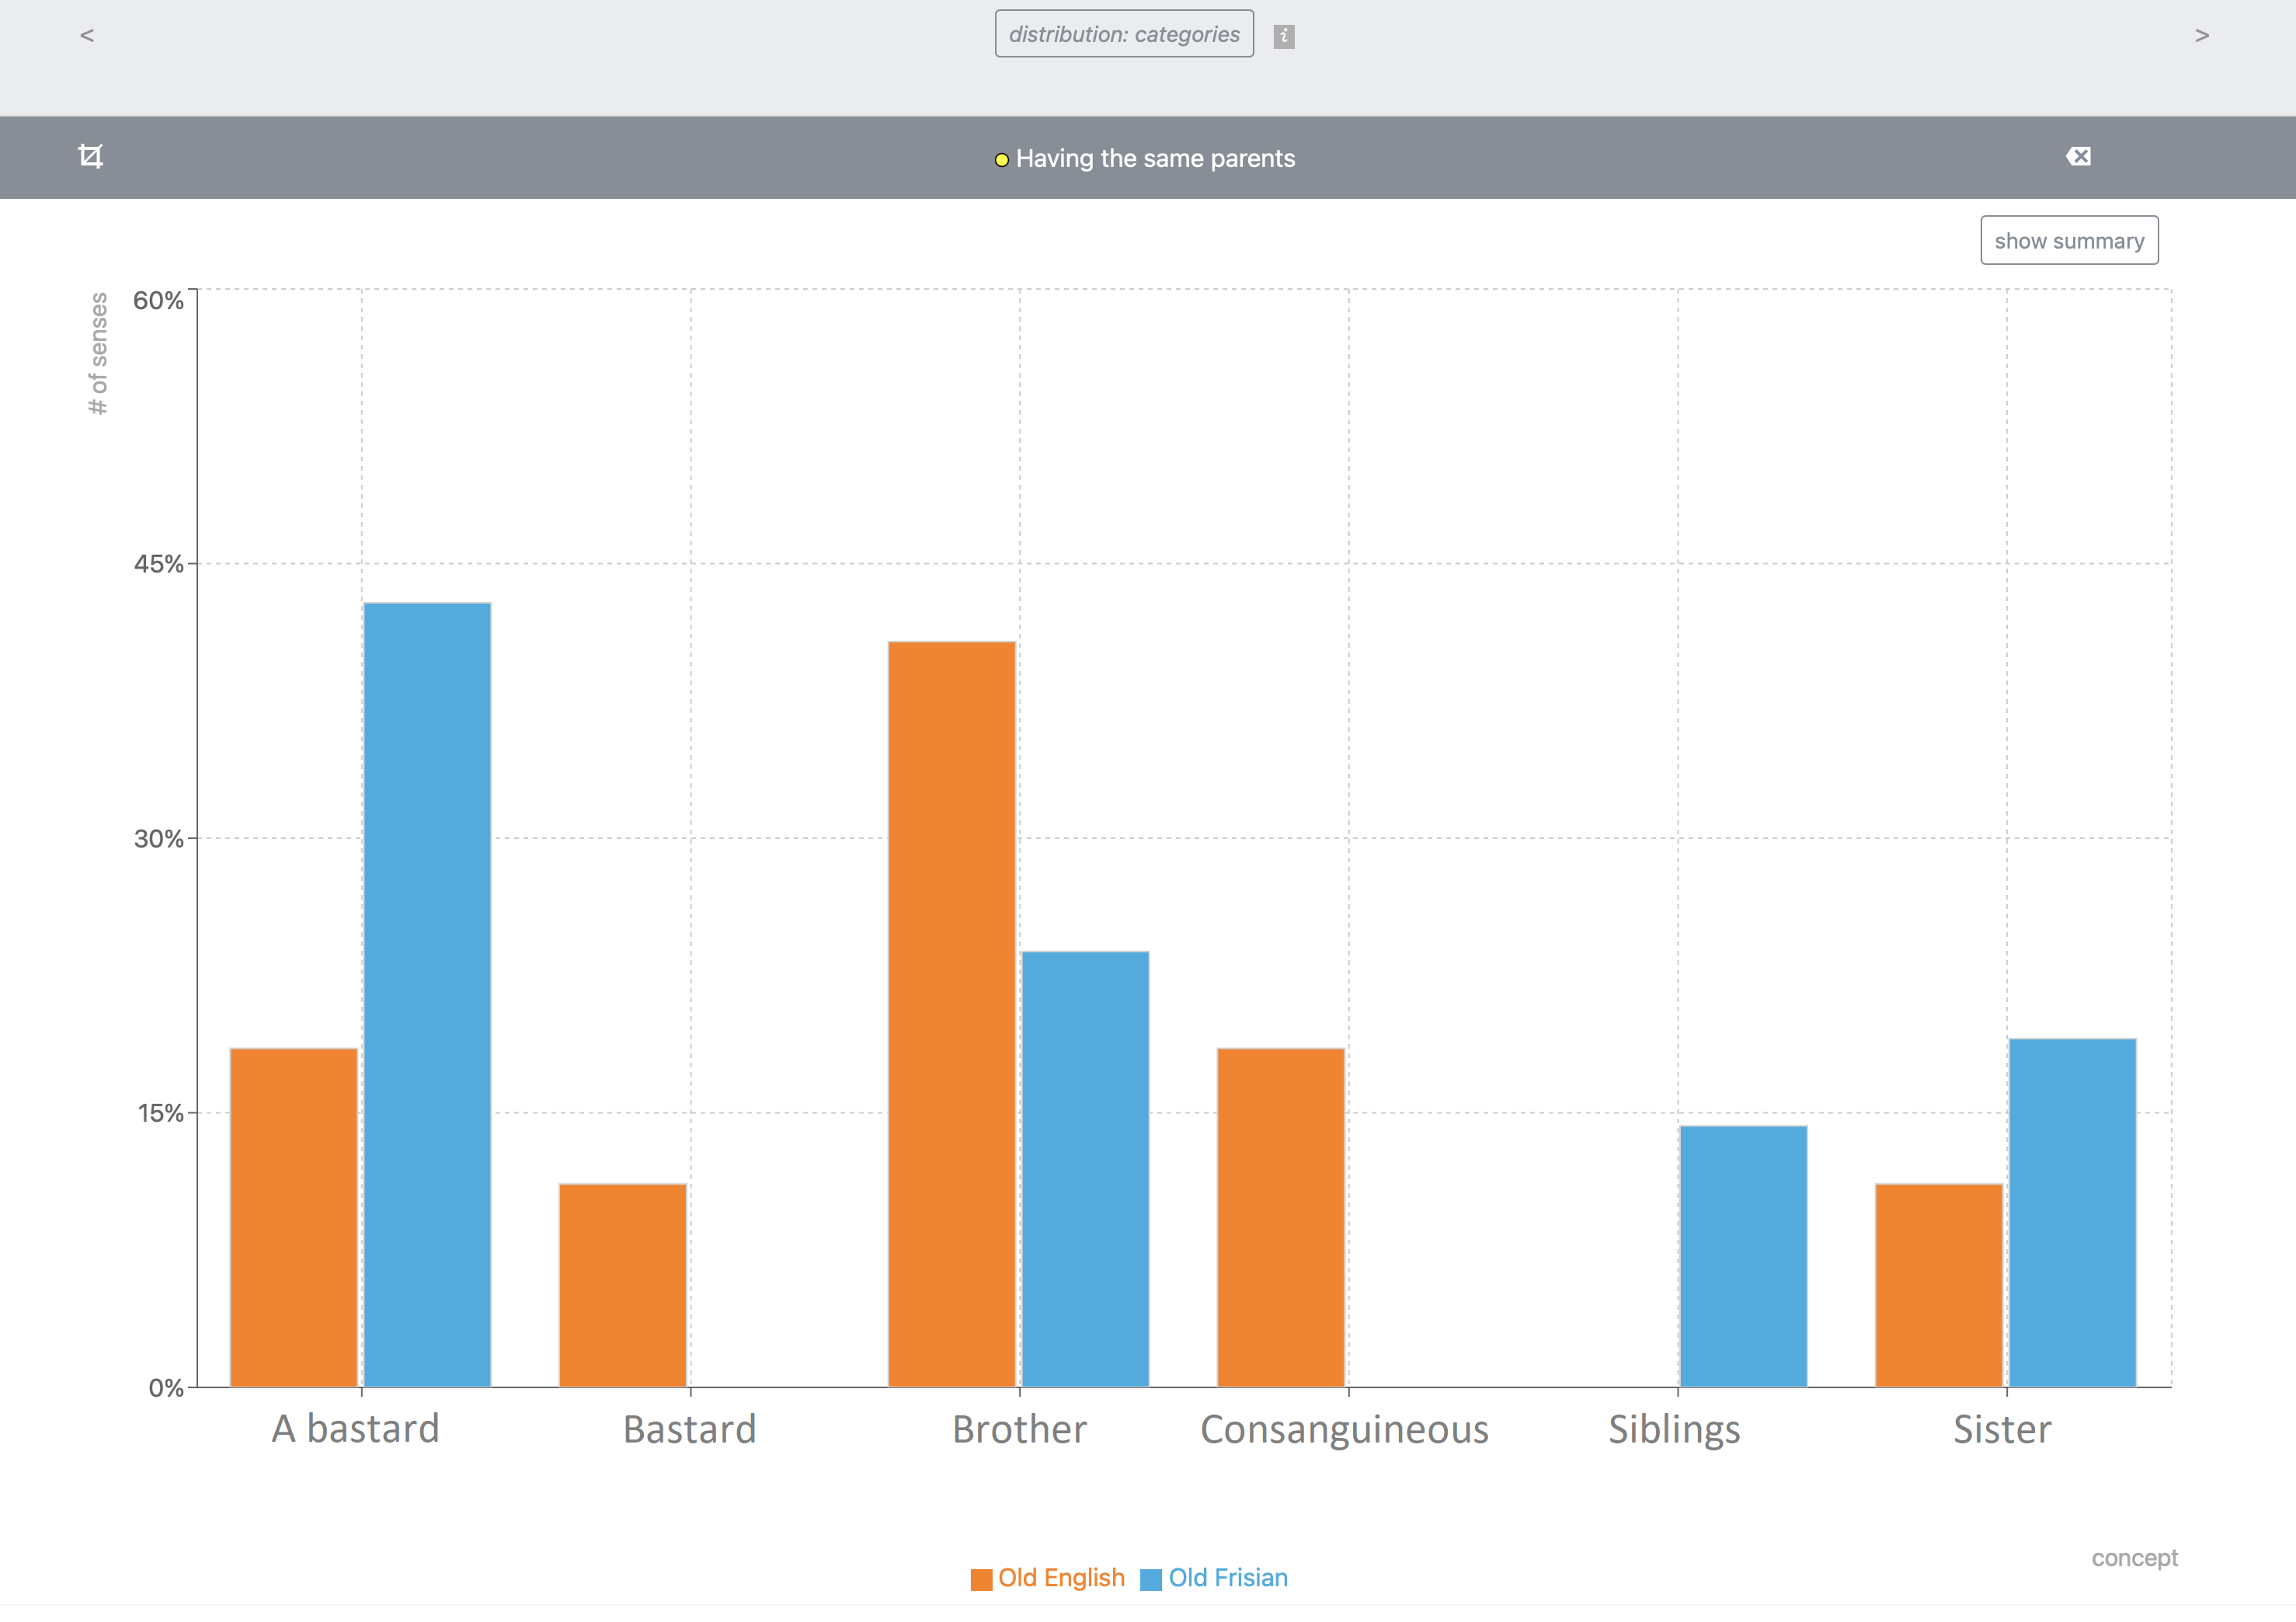
\includegraphics[width=\textwidth]{Stolk2021b/fig/Fig9.png}
	\caption[]{\label{fig:Stolk2021b:Fig9} Distribution of lexical senses over the semantic subfields of “02.03.02.02.05 Having the same parents”.}
\end{figure}


\section{Discussion}
\label{sect:Stolk2021b:Discussion}

The analyses and results in the previous sections are to be read in the context of the languages and resources that lie at their heart. Old Frisian and Old English are not contemporaneous languages: the surviving sources for Old Frisian are coeval with the period of Middle English. The observed contrasts in comparing these languages, however similar they may be, will therefore likely be influenced by the temporal as well as regional space between them. Likewise, it is important to bear in mind the nature of the corpora from which the lexicon was reconstructed. Surviving texts represent but a small portion of what must have been written, by a non-homogeneous group, and, perhaps more importantly, solely by those who were literate. Religious and administrative texts therefore represent a large portion of these medieval corpora, with certain genres more dominant than others (e.g., homilies in Old English, legal documents in Old Frisian).

The alignment of Old Frisian senses with the semantic hierarchy of TOE was complicated by differences between the lexicographic resources used (i.e. AFWB for Old Frisian and TOE for Old English) and the cultural contexts in which they were created. AFWB and TOE use different languages and practices to describe their lexicon: the former employs Modern German to define senses, the latter Modern English; AFWB is a concise dictionary; TOE is based on more detailed dictionaries and demands sense differentiation to be of use. Allocating senses from one language to a taxonomy of a resource created for another, then, is by no means straightforward (see Appendix 1 for notes). As a result, observations with lingual comparisons, such as those made in this article, reflect differences between not only the language communities concerned, but also between the lexicographic practices that contributed to the frameworks used for interpretation of the lexis.

\section{Conclusion}
\label{sect:Stolk2021b:Conclusion}

In this study we set out to answer two questions. The first is whether it is possible to allocate the Old Frisian lexis within the semantic field of \textsc{kinship} to the onomasiological macrostructure of TOE. The answer is in the affirmative. We have demonstrated that Old Frisian senses for \textsc{kinship} can be viewed in an onomasiological structure, alongside Old English ones, by reusing the TOE macrostructure. However, the process of allocating senses from one language to a taxonomy of a resource created for another is by no means straightforward, as mentioned before. In addition to differences between the lexicographic practices for the two resources that have been aligned, a substantial number of Old Frisian senses, owing to their specialized meaning, demanded new categories to be fashioned and positioned into the taxonomy of TOE. For the domain of \textsc{kinship}, these newly created categories could be slotted into lower, more specialized levels of the semantic hierarchy of TOE. The current research does not yet allow us to establish whether reuse and extension of an existing onomasiological structure was more time efficient than building one from the ground up. Of course, creating a new hierarchy, rather than reusing that of TOE, would have the disadvantage of forestalling onomasiological comparisons between Old Frisian and Old English. We surmise that adoption of semi-automated approaches (e.g., automated recognition of cognates) may be used in the future to significantly speed up the alignment process. 

The second question that we have aimed to answer is whether Evoke, in combination with TOE, can offer new insights both for Old Frisian and, in contrast to Old Frisian, Old English. As demonstrated, there are a number of advantages to having Old Frisian lexis available in the onomasiological structure of a thesaurus. The first is that the resulting resource facilitates word field studies (comparable to those for which TOE has been used in the context of Old English) and comparative linguistic research (see the Results section). In fact, we expect the Old Frisian lexis to be accessible to a larger audience through Evoke, owing to the availability of Old Frisian senses in a digital resource that contains Modern English headings, using the TOE macrostructure, rather than in a dictionary that records sense definitions in German. A second advantage is that statistical analyses such as those enabled by Evoke lead to new knowledge of Old Frisian lexis. Preliminary analyses have already demonstrated that the field of \textsc{kinship} in the surviving Old Frisian lexis consists of significantly fewer adjectives and more verbs compared to Old English; it contains lemmata that are mostly monosemous (90\%); it includes more fine-grained senses than Old English (including ones to denote different degrees of kinship); it has a relatively higher degree of lexicalization of the concepts of ancestry and descent than Old English; but it lacks any words for the concepts of adoption, foundling, twins, and triplets. Findings in Evoke lead to new questions that merit further research – into the surviving corpus and lexicographic practices, amongst others – to supply a satisfying context and better understanding. The availability of both Old Frisian and Old English lexis in Evoke, then, certainly offers a useful stepping stone to learn more about the nature of these kindred historical languages and their language communities.

\section{References}

AFWB = Hofmann, D., and A. T. Popkema. Altfriesisches Handwörterbuch (Heidelberg: Universitätsverlag Winter, 2008).
Bajema, I. M. “The Mother’s Brother: An Investigation into the Meaning of Old English Eam.” Neophilologus 78 (1994), 633-643.
Baker, P. S. Introduction to Old English (Chichester: Wiley-Blackwell, 2012).
Baldi, P. Linguistic Change and Reconstruction Methodology (Berlin and New York: De Gruyter Mouton, 2011).
Bammesberger, A. “Altfriesisch swâger.” Indogermanische Forschungen 73 (1968), 133-135.
Boersma, U. J. “De frou yn 'e Fryske wetten.” Us Wurk 10 (1961), 58-85.
Boutkan, D., and S. Siebinga. Old Frisian Etymological Dictionary (Leiden: Brill, 2005).
Bremmer Jr, R. H. “Insults Hurt: Verbal Injury in Late Medieval Frisia.” In Approaches to Old Frisian Philology, eds. R. H. Bremmer Jr, T. S. B. Johnston, and O. Vries (Amsterdam: Rodopi, 1998), 89-112.
Bremmer Jr, R. H. “Language and Contents of the Old Frisian Manuscripts from Rüstringen (c.1300): A ‘Veritable Mixtum Compositum’.” In Advances in Old Frisian Philology, eds. R. H. Bremmer Jr, S. Laker and O. Vries (Amsterdam: Rodopi, 2007), 29-64.
Bremmer Jr, R. H. “Taking Stock of Old Frisian Studies: 1992-2021.” Us Wurk (2021), 1-28.
Bremmer Jr, R. H. “The Importance of Kinship: Uncle and Nephew in Beowulf.” Amsterdamer Beiträge zur älteren Germanistik 15 (1980), 21-38.
Bremmer Jr, R. H. A Bibliographical Guide to Old Frisian Studies (Odense: Odense UP, 1992).
Bremmer Jr, R. H. An Introduction to Old Frisian: History, Grammar, Reader, Glossary (Amsterdam: John Benjamins Publishing Company, 2009).
Chandler, D. and R. Munday. A Dictionary of Media \& Communication, 2nd edn (Oxford: Oxford University Press, 2016).
Colleran, R. A. B. Keeping it in the Family. Disentangling Contact and Inheritance in Closely Related Languages. Doctoral Dissertation (The University of Edinburgh, 2017).
Dance, R. Review of TOE, Medium Ævum 66 (2) (1997), 312-313.
Díaz-Vera, J. E. “Reconstructing the Old English Cultural Model for Fear.” Atlantis 33 (2011), 85-103.
Diepeveen, A. “Verwantschapstermen in de Germaanse Talen.” Antwerp Papers in Linguistics 105 (Universiteit Antwerpen, 2003).
Durkin, P. “New Light on Early Middle English Borrowing from Anglo-Norman: Investigating Kinship Terms in grand-.” Anglia 137 (2019), 255-277.
DWDS = Digitales Wörterbuch der deutschen Sprache (Berlin: Berlin-Brandenburgischen Akademie der Wissenschaften), https://www.dwds.de/d/wb-dwdswb.
Evoke = Stolk, S. Evoke (Web application, 2018), http://evoke.ullet.net/.
Fischer, A. “Of Fæderan and Eamas: Avuncularity in Old English.” In The Power of Words: Essays in Lexicography, Lexicology and Semantics in Honour of Christian J. Kay, eds. G. D. Caie, C. Hough and I. Wotherspoon (Amsterdam: Rodopi, 2006), 67–77.
Fox, R. Kinship and Marriage: An Anthropological Perspective, 2nd edn (Cambridge: Cambridge UP, 1984).
Friel, B. M., and S. M. Kennison. “Identifying German-English Cognates, False Cognates, and Non-Cognates: Methodological Issues and Descriptive Norms.” Bilingualism: Language and Cognition 4 (3) (2001), 249–74.
Görlach, M. Review of TOE, Anglia 116 (3) (1998), 398-401.
Hofmann, G., ed. Mittelalterliches Alltagsleben im Spiegel der altfriesischen Terminologie: mit Ergänzungen aus zeitgenössischen niederländischen Quellen, Estrikken 98 (Kiel: Nordfriesische Wörterbuchstelle Christian-Albrechts-Universität, 2015).
Hough, C. “Old English weargbeorg.” Notes and Queries 54 (4) (2007), 364-365.
Kok, W. “Houlik en earberens by us forfaers.” It Beaken 9 (1947), 59-64, 67-73.
Lancaster, L. “Kinship in Anglo-Saxon Society: I.” The British Journal of Sociology 9 (1958), 230-250.
Lancaster, L. “Kinship in Anglo-Saxon Society: II.” The British Journal of Sociology 9 (1958), 359-377.
Lowe, K. A. “Never Say Nefa Again: Problems of Translation in Old English Charters.” Neuphilologische Mitteilungen 94 (1993), 27-35.
Loyn, H. R. “Kinship in Anglo-Saxon England.” Anglo-Saxon England 3 (1974), 197-209.
Meijering, H. D. Chindh uuirdit uns chiboran. Over het woord ‘kind’ in het oudere Duits (Amsterdam: Vrije Universiteit, 1985).
Meijers, E. M. “Eine germanische Zählung der Verwandtschaftsgrade.” Tijdschrift voor Rechtsgeschiedenis 6 (1925), 1-52.
Munske, H. H. Der germanische Rechtswortschatz im Bereich der Missetaten: Philologische und sprachgeographische Untersuchungen. I: Die Terminologie der älteren westgermanischen Rechtsquellen (Berlin: De Gruyter, 1973).
Munske, H. H. et al., eds. Handbuch des Friesischen. Handbook of Frisian studies (Tübingen: Max Niemeyer Verlag, 2001).
Ojanguren López, A. E. “Old English Try Verbs: Grammatical Behaviour and Class Membership.” Studia Neophilologica (2021), 1-19.
Otwinowska-Kasztelanic, A. “Awareness and Affordances: Multilinguals Versus Bilinguals and Their Perceptions of Cognates.” In New Trends in Crosslinguistic Influence and Multilingualism Research, eds. G. De Angelis and J. M. Dewaele (Bristol and Blue Ridge Summit: Multilingual Matters, 2011), 1-18.
Pfeffer, G. “The Vocabulary of Anglo-Saxon Kinship.” L’Homme 27 (1987), 113-128.
Popkema, A. T. “Die altfriesischen Eidesbezeichnungen.” In Advances in Old Frisian Philology, eds. R. H. Bremmer Jr, S. Laker and O. Vries (Amsterdam: Rodopi, 2007), 325-356.
Pospelova, K. “Old Frisian Compounds: Kinship Terms.” Žmogus ir Žodis 19 (2018), 79-96.
Rauer, C. “Mann and Gender in Old English Prose: A Pilot Study.” Neophilologus 101 (1) (2017), 139-158.
Roberts, J. “Towards an Old English Thesaurus.” Poetica 9 (1978), 56-72.
Salmons, J. “What Old Frisian Can Tell Us about the History of i-Umlaut across West Germanic?” In Advances in Old Frisian Philology, eds. R. H. Bremmer Jr, S. Laker, and O. Vries (Amsterdam: Rodopi, 2007), 367-377.
Schmitt, N. “Vocabulary Learning Strategies.” In Vocabulary: Description, Acquisition and Pedagogy, eds. N. Schmitt and M. McCarthy (Cambridge: Cambridge UP, 1997), 199-227.
Scott, P. “Conceptualising Olfaction: A Study of the Scent Nouns and Adjectives in Old English.” Studia Neophilologica (2021), 1-18.
Sjölin, B. “Zur Gliederung des Altfriesischen.” Us Wurk 15 (1966), 25-38.
Spolsky, E. “Old English Kinship Terms and Beowulf.” Neophilologische Mitteilungen 78 (1977), 233-238.
Sterringa, A. “The Most Miserable Women of all: Widows in Medieval Frisia.” In Approaches to Old Frisian Philology, eds. R. H. Bremmer Jr, T. S. B. Johnston, and O. Vries (Amsterdam: Rodopi, 1998), 285-301.
Stroh, F. Handbuch der germanischen Philologie (Berlin: De Gruyter, 1985).
Tissari, H. “Current Emotion Research in English Linguistics: Words for Emotions in the History of English.” Emotion Review 9 (1) (2017), 86-94.
TOE = Roberts, J., and C. Kay with L. Grundy. A Thesaurus of Old English (Glasgow: University of Glasgow, 2017), http://oldenglishthesaurus.arts.gla.ac.uk/.
Trask, R. L. Trask’s Historical Linguistics, ed. R. McColl Millar. 3rd edn (London and New York: Routledge, 2015).
Van de Poel, R. Corpus Oudfries (2019), http://corpora.ato.ivdnt.org/corpus-frontend/OFR/.
Versloot, A. P. “Mechanisms of Language Change: Vowel Reduction in 15th Century West Frisian.” Doctoral dissertation (University of Groningen, 2008).
Versloot, A. P. “Why Old Frisian Is Still Quite Old.” Folia Linguistica Historica 38 (2004), 253-298. 
Vries, O. “Die altfriesischen Urkunden.” In Handbuch des Friesischen. Handbook of Frisian studies, eds. H. H. Munske et al. (Tübingen: Max Niemeyer Verlag, 2001), 594-601.
Wierzbicka, A. Understanding Cultures through Their Key Words: English, Russian, Polish, German, and Japanese (Oxford: Oxford University Press, 1997).
Zeilfelder, S. “Das Wortfeld ‘Mensch’.” In Deutsche Wortfeldetymologie in europäischem Kontext, Band 3: Mensch und Mitmensch, ed. R. Lühr (Wiesbaden: Reichert, 2015), 33-110.

\section{Appendix 1: Notes on the alignment}
This appendix provides notes on the alignment between the Altfriesisches Handwörterbuch (AFWB) and A Thesaurus of Old English (TOE) for the semantic field of \textsc{kinship}.

1) AFWB lemmata or senses discarded or updated

•	The second sense recorded in AFWB for evenknē, i.e. “Verwandter” [relative], is disputable and has therefore been discarded.
•	Senses recorded in AFWB for bern and kind do not reflect that they are synonyms. With the help of the online corpus of Old Frisian, it is easy to find instances that attest to the conclusion that bern and kind have the same senses, i.e. 1) Foetus, 2) Offspring (first degree), 3) Descendant and 4) Young, immature person. We have therefore chosen to align the senses of bern and kind with each other.
•	The recorded sense in AFWB for unnatlik, i.e. “unebenbürtig” [not equally related], is inaccurate and should be “not related.”
•	The senses of Old Frisian kennemech has been aligned with those of keremech.

2) Lemmata or senses introduced

The following terms were not recorded in AFWB but are attested in the Old Frisian corpus and were added to the dataset used in this article.

•	sex honda as a phrase with the sense “First degree blood relatives”.
•	thredda as a noun with the sense “Third generation”.

The phrase sex honda is found in 7 manuscripts, in one of the most widely distributed texts known as the Twenty-four Land Laws.  Thredda is recorded in the AFWB as numerical form with the general sense of dritte [third], but the more specialized sense of “third generation” is also recorded in the Old Frisian sources. 

3) Remarks on placement of senses in TOE

•	Definitions in AFWB of a number of Old Frisian senses on \textsc{kinship} contained elements that made it possible to allocate these senses to fields outside of \textsc{kinship}, too. Instead of allocating them to multiple semantic fields, these senses were allocated solely to categories in \textsc{kinship}. The Old Frisian lemma kniaia, for instance, has a sense of “lawfully claiming to be related”. This sense was allocated to \textsc{kinship} in TOE only, but not additionally to the semantic field of “14.03.03 n. Law, action of the courts”.  Similarly, lemmata with the sense of “being related” or “relationship” were not allocated to the semantic field of “08.01 n. Heart, spirit, mood, disposition” in TOE. 
•	The AFWB lemma kniaia has three overlapping senses: “Verwandschaft nachweisen,” “Verwandschaft geltend machen,” “verwandt sein.” We merged these three into one sense in English: “To (claim to) be related.”
•	Senses defined as “Blutverwandt” or “Verwandt” are used indiscriminately in the AFWB. These senses have all been aligned as “Related.” Similarly, the AFWB uses “Blutverwandtschaft” and “Verwandtschaft” indiscriminately. Blood relations and blood relatives all belong to TOE category “Close relationship.”

4) Comments on the structure of TOE 

In the following paragraphs we illustrate some of the difficulties experienced when placing the Old Frisian senses from AFWB within the categories from TOE.

•	The AFWB records a single sense for the Old Frisian lemma dochter with its definition in German: “Tochter” [daughter]. TOE records the Old English cognate dohtor in different senses: one is listed in the category “02.03.02.02.04 A daughter”, another in the category “02.03.02.03.05 | 02 n. Female descendant”.  The Old Frisian lemma's meaning refers to both of these. The question arises as to whether one should allocate the single recorded sense of Old Frisian dochter to the same two categories as Old English dohtor. Since it is obvious that a daughter is also a female descendant, a sense that is also part of \textsc{kinship}, we have decided to allocate the recorded sense in AFWB to both categories. An alternative solution would be to create two subsenses of the AFWB lemma and have allocated these to their respective categories.
•	The senses of the cognate words Old English fǣmne and Old Frisian fomne are related but still slightly different:

Lemma 	TOE categories
Old English fǣmne	Female person, woman	Girl	A maiden, A virgin
	AFWB senses
Old Frisian fomne	1) Mädchen [girl]	2) Tochter [daughter]	3) Magd [female servant]

When looking at the TOE categories for fǣmne, the category “02.03.01.02 Female person, woman” is a sense more general than those recorded in AFWB.  Although the lemma may fit in this category, too, we have decided to keep the three senses recorded in AFWB unchallenged, positioning only these in the semantic hierarchy of TOE on \textsc{kinship}.

5) Inconsistencies AFWB

The senses of (near-)synonyms and other semantically related words have some inconsistencies. Cases in point are Old Frisian wīf and frouwe.

	wīf n. 1) Weib; 2) Frau 
	frouwe, frowe, frouWL f. 1) Frau; 2) Ehefrau; 3) Edelfrau, Fürstin; 4) Herrin; 5) die Jungfrau 
	Maria; 6) Schwiegermutter 

Examination of the contexts in which the lexemes wīf and frouwe occur reveals that the compilers of the AFWB have tried to reflect the connotational differences that the two words have in the German descriptions. Frouwe was a term used to denote respect, while wīf was the more generally used word. For frouwe only the senses 1, 2 and 6 have been allocated to \textsc{kinship} in TOE (the others fall outside the scope of our investigation). Corresponding TOE categories are “02.03.01.02 Female person, woman” and “12.09 | 07.05 n. Wife, married woman.” 

6) Allocation of AFWB senses to multiple TOE categories

Six senses from AFWB have been allocated to not one but two TOE categories, effectively creating two subsenses for each of these AFWB senses when assigning them to the onomasiological structure of TOE. The allocation to a second TOE category allowed, most notably, for words denoting offspring (such as “son” or “daughter”) to be marked as “descendant”, too. The six AFWB senses, along with their allocations in TOE, are as follows:

	
AFWB	TOE
lemma	senseno.	sense	Mod. English translation	category 1	category 2
dochter	1 	Tochter	daughter	A daughter  	Descendant 
kind	2 	Kind, Nachkomme	child, descendant	Child, offspring 	Descendant
knapa	2 	Sohn	son	A son 	Descendant
sunder\_1	1	Sohn	son	A son	Descendant
sune	1	Sohn	son	A son	Descendant
slachte\_1	2	Familie	family	Ancestry 	Kinsman/relative 

\section{Appendix 2: Old Frisian lemmata on kinship aligned with A Thesaurus of Old English}
Categories in italics are ones that did not exist in the original thesaurus taxonomy and have been newly created to accommodate Old Frisian senses.

02.03.02 Family/household (id: 1108) 
IRI: \url{https://oldenglishthesaurus.arts.gla.ac.uk/category/#id=1108}

02.03.02.01 Parent (1109)	alder
	01 n. Father (1110)		feder
	02 n. Mother (1112)	mōder
	
02.03.02.02 Child, offspring (1113)		bern, kind
	04 adj. Lawfully born (1120)		aftberen
	06 n. An orphan (1124)		wēsa, wēsekin, wēsekind, wēseklēn, wēstien
		02 adj. Without Parents (1126)		alderlās, biwēsed, wēsid
		05 adj. For orphans		wēslik
	02.03.02.02.03 n. A son (1131)		knapa, sunder, sune
02.03.02.02.04 n. A daughter (1133)		fomne, dochter

02.03.02.02.05 Having the same parents (1136)		
02 n. A Bastard (1141)		basterd, hōringe, hōrkind, hōrning, hōrbrēd, hōrbern
		02 n. Bastard brother (1143)		basterdbrōther
		03 n. Bastard sister		basterdswester
		04 n. Bastard born before marriage	spilkind
02.03.02.02.05.01 Brother (1146)		brōther
		06 adj. Of brothers, brotherly (1154)		brōtherlik
		06.01 n. State of being brotherly		brōtherlikhēd
		08 n. Full brother		fulbrōther
		09 n. Half brother		halfbrōther
02.03.02.02.05.02 Sister (1156)		swester
		01 n. Full sister		fulswester
		02 n. Half sister		halfswester
		02 n. Sisterhood		swesterskip
		02.03.02.02.05.03 Siblings 		swesterne
			01 n. Full siblings		fulswesterne
			02 n. Half siblings		halfswesterne

02.03.02.03 Ancestry, descent (1159)		slachte
	02 Side (1162)		sīde
03 Generation, degree of descent (1163)		grād, gung, knī, lith, sibdēl, siā, slachte, sibdēl
	02 Third generation		thredda
	03 Descendance		delgung, nithergung, tōdele
		01 v. To descend		delgunga, nithergunga, tōdelgunga
		02 adj. Descending, down		delgungande
		03 adv. Descendingly		tōdele
	04 Ascendance		upgung
		01 v. To Ascend		upgunga, ūrbekgunga
		02 adv. Ascendingly, backwards, up	ūrbek
	05 Part of a family tree		facht
	06 Trunk of a family tree		stipa

02.03.02.03.01 Ancestry, paternal kinship (1166)
		02 Male line of descent (1169)		sperehond, swerdsīde
		03 Father's side (1170)		federsīde
			01 Paternal adj (1171)		fetherlik
			02 n. Father's mother side		federesmōdersīde
02.03.02.03.02 Maternal descent (1172)
		02 Female line of descent (1174)		spindelsīde
		03 Mother's side (1175)		mōdersīde
			01 adj. Maternal (1176)		mōderlik
		04 n. Mother's father side		mōderfedersīde

02.03.02.03.03 Forefather, ancestor (1178)		alder, forefeder, forefirdera
	
02.03.02.03.04 (Of degrees of descent) great-, grand- (1182)
01 n. Grandfather (1183)		aldafeder, alder, edela
02 n. Grandmother (1184)		aldemōder,
		03 n. Great grandfather (1185)		ūraldafeder, alder, edela
		04 n. Great grandmother (1186)		ūraldemōder
		09 n. Granduncle		aldaēm

02.03.02.03.05 Descendant (1191)		bern, kind, knapa, neikuma, neikumande,
 					neikumeling, neikumer, sunder, sune
		01 n. Descendants (of a generation) (1192)		neikuminge
		02 n. Female descendant (1193)		dochter
		03 n. Successor, heir (1194)		outside of current scope
		04 n. Grandson (1195)	-
			01 n. Daughter's son (1196)		dochtersune
		12 n. Grandchild		bernesbern, kindeskind
			01 n. Daughter's child		dochteresbern
		13 n. Great grandchild		kindeskindeskind

02.03.02.03.06 Kinship, relationship (1204)		sibbe\_1, blōd, wirtel
01 adj. Related (1205)		bisib, bisibbed, sibbe\_2, swēs, liāf, nātlik

02.03.02.03.06.01 Kinsman, relative (1208)		sibba, sibdēl, kniā, knīling, mēch, friund, nāt, holda
03 n. Paternal relative (1212)		federfriund, federmēch, federsibbe
04 n. Maternal relative (1213)		mōderfriund, mōdermēch
07 n. Next of kin (1216)		nesta
09 n. Kinsfolk (1218)		sibbe\_1, slachte, ken
		05 n.Relationship through common parents		fulsibbe
				01 adj. Rel through common parents				fulsibbe
06 n. Relationship by one parent				halfsibbe
		11 n. Third degree relative		thredkniā, thredknīling, thredling, thredsiā
		12 n. The six first degree relatives		sex honden
		13 n. Relative in the same degree		evenknē, evenkniā, evenknīling, līkenisse
		14 n. Relative chosen for oath swearing		keremēch, kestfriūnd
		15 n. Relative in ascending line 		upstīger
		16 n. Relative in descending line 		nītherstīger

02.03.02.03.06.02 Close relationship (1224)		
01 adj. Closely related (1225)		biefta, inlik, niār
		02 adj. Like relatives		swēslik	
	03 n. Blood relations (1230)		blōd, bērena blōd	
04 adj. Not related (1233)		fremede, unnātlik
05 v. To (claim to) be related		kniāia
		01 v. to (claim to) be closer related		bikniāia, ūrkniāia, ūtsteka
06 adj. Nearest related		allerswesest, allersibbest, nest
07 adj. Too close related (incest)		sibbe\_2
08 adj. More distantly related	ūtlik

02.03.02.03.06.02.01 Uncle (esp. maternal) (1234)	ēm, mōderesbrōther
		01 n. Paternal uncle (1235)		federia
			01 n. Father's halfbrother		halffederia

02.03.02.03.06.02.02 Aunt (1236)			
		01 n. Maternal Aunt (1237)		mōdire, mōie
		02 n. Paternal Aunt (1238)		fethe, federesswester

02.03.02.03.06.02.03 Child of brother/sister (1239)	swesternabern
		01 n. Sister's child (1240)		swesterbern, swesterling, swesterkind
		02 n. Nephew (1241)		neva
			01 n. Sister's son (1242)		swestersune
			02 n. Brother's son (1243)		brōthersune, neva
		03 n. Niece (1244)		nifte, nifke
			01 n. Brother's daughter (1245)brōtheresdochter
			02 n. Sister's daughter		swesterdochter
				03 n. Niece's child		niftlin, niftakind
		05 n. Brother's child		brōtheresbern, brōthereskind
	
02.03.02.03.06.02.04 Cousin (1247)			
		02 n. Father's sister's son (1249)		fethansune
		04 n Relationship between cousins		berning, swire
		05 n. Mother's brother's son		ēmka, ēmessune
		06 n. Mother's sister son		mōdiransune
		07 n. Father's brother's son		federiasune
		08 n. Children of cousin		efterswesterling, efterswesternabern,
 			ōtherswesterbern

02.03.02.03.06.02.05 Step relationships (1251)
		01 n. Step-father (1252)		stiāpfeder
		02 n. Step-mother (1253)		stiāpmōder
		03 n. Step-son (1254)		stiāpsune
		04 n. Step-daughter (1255)		stiāpdochter
		05 n. Step-child		stiāpkind

02.03.02.03.06.02.06 In-law relationships	(1256)	
01 n. Father-in-law (1257)		hēra, swāger
02 n. Mother-in-law (1258)		frouwe
03 n. Daughter-in-law (1259)		snore
	01 n. Being a daughter-in-law	snōrskip
04 n. Brother-in-law (1260)		tāker, āthum
06 n. Son-in-law / brother-in-law (1262)	āthum
07 n. Son-in-law and father-in-law (1263)	siāring
08 n. Son-in-law		swiāring, swāger, dochtermon
 	01 n. Being a son-in-law 	swāgerskip
			09 n. Parents-in-law		swiāring

02.03.02.04 Adoption (1264)	- 
02.03.02.04.01 Foster relationships (1268)		-

02.03.02.05 Spiritual relationships (1274)		fadersibbe, faderskip
	01 adj. Spiritual (1275)		gāstlik
		02.01 n. A godfather (1277)		fadera
	05 n. Relationship betw. godbrother and biological brother	brōtherlikhēd
	06 n. Relationship betw. godfather and biological father	fēderlikhēd


Other TOE categories containing Old Frisian lemmata
As mentioned in section 5, a number of Old Frisian lemmata on \textsc{kinship} have been classified within TOE outside of the semantic field “02.03.02 Family/household”, and are therefore not included in our current analyses and case studies. The classification of these 47 lemmata is provided below.
 
02.01 Existence, life (id: 661) 
IRI: \url{https://oldenglishthesaurus.arts.gla.ac.uk/category/#id=661}

02.01.03 Fruitfulness, fertility (698)
	02.01.03.05 To be fruitful, to produce (705)		forthbrenga

02.01.03.02 Barrenness, sterility (717)
	02 adj. Barren, unproductive (719)		tochtalās

02.01.03.03.01 To beget (730)
	02 n. Begetting of children (732)		berntām, berntochta
	06 n. An embryo/foetus (738)		berde, bern, kind
	09 adj. Pregnant (742)		bernheftich
	12 adj. Childless (745)		bernlās

02.01.03.03.02 To bring forth, produce (747)		
	05 n. Produce, fruit, offspring (752)		frucht

02.01.03.03.03 Birth (761)		berde
	01 v. To be born (762)		bera\_1
	02 adj. Born (763)		beren

	02.01.03.03.03.01 Child-bearing, childbirth (768)	tām
		07 n. A miscarriage (776)		bernwendene, berdwendene, dāden frucht

	02.01.03.03.04 Offspring, race, breed, family, children (780)	not included
	01 n. Progeny, offspring (781)		tām
		02 n. Descendants, progeny, race (784)		not included

	01.01.03.03.06 Sex, kind (789) 		
	01 n. A sex (789)
		01.01 n. A Male (793)		mon
			02 n. Female sex (794)
				01 n. A Female (795)		frouwe, wīf


02.03 Humankind (id: 1059) 		geslachte, slachte\_1
IRI: \url{https://oldenglishthesaurus.arts.gla.ac.uk/category/#id=1059}

02.03.01 People (1065)		menneska
	01 n. Human being (1066)		mon, menneska
	09 v. To have (a brother, husband etc.) (1075)		habba

	02.03.01.01 Male person, man (1076)		mon, hēra, monnesnoma, monnespersōne
		02 adv. In a male manner (1078)		monlike

	02.03.01.02 Female person, woman (1079)		frouwe, wīf, wīfke, wīfnama, menneska, 
				frouwespersōna
		03 adj. Female (1082)		frouwelik, wīflik

02.03.01.04 Child (1086)		kind, kintien, mach, bern
		05 n. Male child (1091)		knapabern, knapakind
		06 n. Female child (1092)		fomnabern, fomnakind

02.03.01.05 Youth, boy, stripling (1093)		knapa, mage

02.03.01.07 Girl (1099)		famke, fomne, megeth, meiden

	12.09 Marriage, state of marriage (id: 18602)
IRI: \url{https://oldenglishthesaurus.arts.gla.ac.uk/category/#id=18602}

06 n. Married persons, married couple (18610)		hiūne, sinhīgen
07.03 n. Husband, (married) man (18615)		mon
07.05 n. Wife, married woman (18618)		wīf, wīfke, wīfnama, hūsfrouwe
	
12.09.03 Unmarried state (18657)
		02 A maiden, a virgin (18663)		megeth
		03 An unmarried man (18665)		knapa

12.09.05 State of a woman whose husband has died (18683)
		01 Relict, widow (18684)		widwe
		02 Widower (18685)		wedener

